\chapter{Formulaci'on Covariante de la Electrodin'amica}

\section{Conservaci'on de la carga el'ectrica y ecuaci'on de continuidad}\label{ccer}

En el vac'io (es decir, en ausencia de un medio material) las ecuaciones de Maxwell pueden escribirse ($c^2=1/\varepsilon_0\mu_0$) como:
\begin{equation}\label{inrho}
\vec{\nabla}\cdot \vec{E} = \mu_0 c^2\rho ,
\end{equation}
\begin{equation}\label{inj}
\vec{\nabla}\times \vec{B} = \frac{1}{c^2} \frac{\partial \vec{E}}{\partial t} +\mu_0\vec{J} ,
\end{equation}
\begin{equation}\label{db0}
\vec{\nabla}\cdot \vec{B} =0 ,
\end{equation}
\begin{equation}\label{de+}
\vec{\nabla}\times \vec{E} = - \frac{\partial \vec{B}}{\partial t} .
\end{equation}
Estas ecuaciones se complementan con la expresi'on para la fuerza de Lorentz que, para una carga (puntual) $q$ movi'endose con velocidad $\vec{v}$, asume la forma
\begin{equation}
\vec{F} = q \left( \vec{E} + \vec{v}\times \vec{B}\right) .
\end{equation}
Las ecuaciones de Maxwell implican la ley de conservaci'on de la carga el'ectrica. Usando (\ref{inj}) y (\ref{inrho}) podemos escribir:
\begin{eqnarray}
\vec{\nabla}\cdot (\vec{\nabla}\times \vec{B}) &=& \frac{1}{c^2} \vec{\nabla}\cdot\frac{\partial \vec{E}}{\partial t} + \mu_0 \vec{\nabla}\cdot \vec{J}\\
 &=& \frac{1}{c^2} \frac{\partial (\vec{\nabla}\cdot \vec{E})}{\partial t} +
\mu_0 \vec{\nabla}\cdot \vec{J}\\
&=&\mu_0\frac{\partial \rho}{\partial t} + \mu_0
\vec{\nabla}\cdot \vec{J} ,
\end{eqnarray}
de modo que obtenemos la \textit{ecuaci'on de continuidad} \eqref{eccont}.
%que expresa la conservaci\'on de la carga el\'ectrica ($\int_V \rho dV=\rm cte$
%si $\vec{J}=\vec{0}$ en la superficie $\partial V$).

Deseamos asegurar que la teor'ia electromagn'etica sea compatible con los
principios de la teor'ia de RE y, en particular, con el Principio de Relatividad. Para esto estudiemos c'omo deben cambiar los campos bajo cambios de SRI, de modo que se asegure que las ecuaciones de Maxwell sean v'alidas \textit{con la misma forma} en todo SRI. Esto puede ser realizado si logramos escribir las ecuaciones de Maxwell en t'erminos de 4-vectores y/o 4-tensores.

Por simplicidad, comenzaremos por la ecuaci'on de continuidad (\ref{eccont}). Para asegurar que la ley de conservaci'on de la carga el'ectrica sea v'alida en todo SRI la
ecuaci'on (\ref{eccont}) debe ser covariante bajo TL's.  Dado que
$c^{-1}\partial_t$ y $\vec{\nabla}$ son las componentes de
$\partial_\mu=(c^{-1}\partial_t, \vec\nabla)$, que transforma
como un 4-vector (operador) covariante bajo TL's, podemos escribir
(\ref{eccont}) como
\begin{equation}
\partial_\mu J^\mu=\frac{\partial(c \rho)}{\partial x^0} + \partial_i J^i =0
,\label{dj0}
\end{equation}
donde hemos denotado $J^0:=c \rho $, 
%$J^1:=J_{x}$, $J^2:=J_{y}$, $J^3:=J_{z}$,
de modo que $J^\mu :=(c \rho,J^i)=(c \rho,\vec{J})$.

La invariancia de forma de la ecuaci'on de continuidad estar'a asegurada si el conjunto de 4 cantidades $J^\mu$ \textit{transforma como un vector contravariante bajo TL's}. Llamamos al 4-vector $J^\mu$ la \textit{4-densidad de corriente} o simplemente la \textit{4-corriente}. En efecto, si en un SRI $K'$ tenemos que $x'^\mu=\Lambda^\mu_{\ \nu}x^\nu$ entonces $J'^\mu=\Lambda^\mu_{\ \nu}J^\nu$ adem'as de $\partial'_\mu=(\Lambda^{-1})^\nu_{\  \mu}\partial_\nu$, de modo que $\partial'_\mu J'^\mu=\partial_\mu J^\mu$ (en otras palabras ``la 4-divergencia de la 4-corriente es un escalar") y por consiguiente $\partial'_\mu J'^\mu=0$.

El asumir que las componentes de la 4-corriente (la densidad y las componentes de la densidad de corriente) forman un 4-vector bajo TL's es consistente con la conocida expresi'on $\vec{J}=\rho\vec{v}$, que es v'alida para la densidad de corriente de una
distribuci'on con densidad de carga $\rho$ movi'endose con velocidad $\vec{v}$.
En efecto, si en un SRI $K_0$, com'ovil con (un punto dado de) la distribuci'on de carga, tenemos que $\vec{v}_0=\vec{0}$ y la densidad de carga es $\rho_0$ entonces, \textit{asumiendo} que $\vec{J}^\mu$ es un 4-vector tendremos, usando el boost (\ref{bg1})-(\ref{bg2}), que en otro SRI en el que las cargas se mueven con velocidad $\vec\beta c$ las componente de la 4-corriente ser'an
\begin{equation}
\vec{J}=\gamma\vec\beta J^0=\gamma\vec\beta c \rho_0, \qquad  c\rho=\gamma J^0=\gamma c
\rho_0,
\end{equation}
de modo que $\vec{J}=\rho\vec{v}$. Note que el cambio en la densidad de
carga (carga por unidad de volumen), $\rho=\gamma\rho_0$ es consistente con la contracci'on de longitudes (y por tanto, de volumen) en la direcci'on de movimiento.

Puede verificarse que si $J^\mu$ es un 4-vector
contravariante, entonces \textit{la carga total en un volumen} $V$, $Q=\int_V (J^0/c)dV$ \textit{es un escalar bajo TL's}. Alternativamente, podemos justificar el car'acter
vectorial de la \textit{4-densidad de corriente} $J^\mu$ exigiendo (inspirado en la informaci'on experimental disponible) que la carga el'ectrica sea un escalar.

Note adem'as que para el caso de una distribuci'on de carga con densidad $\rho$ y 4-velocidad $u^\mu$ podemos escribir la 4-densidad de corriente $J^\mu$ como
\begin{equation}
\boxed{J^\mu=\rho_0 u^\mu,}
\end{equation}
donde $\rho_0:={\rho}/{\gamma}$ es un \textit{escalar} que describe la \textit{densidad de carga en el SRI com'ovil con la distribuci'on}: la \textit{densidad propia de carga}.


\section{Ecuaciones de Maxwell inhomog'eneas}

Sabiendo que $J^\mu$ es un 4-vector, podemos analizar las propiedades de transformaci'on de los campos el'ectrico y magn'etico de modo que las ecuaciones de Maxwell inhomogeneas preserven su forma bajo TL's. Podemos escribir (\ref{inrho}) y (\ref{inj})  m'as expl'icitamente como:
\begin{eqnarray}
\frac{1}{c}\frac{\partial E^x}{\partial x} + \frac{1}{c}\frac{\partial E^y}{\partial y} + \frac{1}{c}\frac{\partial E^z}{\partial z} &=& \mu_0\, J^0 , \\
\frac{\partial B^z}{\partial y} - \frac{\partial B^y}{\partial z} - \frac{1}{c^2}\frac{\partial E^x}{\partial t} &=& \mu_0\,  J^1 , \\
\frac{\partial B^x}{\partial z} - \frac{\partial B^z}{\partial x} - \frac{1}{c^2}\frac{\partial E^y}{\partial t} &=& \mu_0\,  J^2 , \\
\frac{\partial B^y}{\partial x} - \frac{\partial B^x}{\partial y} - \frac{1}{c^2}\frac{\partial E^z}{\partial t} &=& \mu_0\,  J^3 .
\end{eqnarray}
Reescribimos estas ecuaciones en la forma siguiente,
\begin{eqnarray}
0 + \partial_1 F^{10} + \partial_2 F^{20} + \partial_3 F^{30} &=& \mu_0\,
J^0 ,\\
\partial_0 F^{01} + 0+ \partial_2 F^{21} + \partial_3 F^{31} &=& \mu_0\,
J^1 ,\\
\partial_0 F^{02} + \partial_1 F^{12} +0+ \partial_3 F^{32} &=& \mu_0\,
J^2 ,\\
\partial_0 F^{03} + \partial_1 F^{13} + \partial_2 F^{23} +0&=& \mu_0\,
J^3,
\end{eqnarray}
o, en forma compacta,
\begin{eqnarray}
\partial_\mu  F^{\mu \nu} = \mu_0\, J^\nu  , \label{coninhom}
\end{eqnarray}
con
\begin{eqnarray}
F^{\mu \nu}:=
\left(
\begin{array}{cccc}
0&-E^x/c&-E^y/c&-E^z/c\\
E^x/c&0&-B^z&B^y\\
E^y/c&B^z&0&-B^x\\
E^z/c&-B^y&B^x&0
\end{array}
\right) . \label{Fupup}
\end{eqnarray}
Es claro de (\ref{coninhom}) que la invariancia de forma de las ecuaciones inhomog'eneas de Maxwell queda asegurada si las 6 cantidades independientes correspondientes a los campos el'ectrico y magn'etico \textit{forman un tensor antisim'etrico} $F^{\mu \nu}=-F^{\nu\mu}$, llamado \textit{tensor de electromagn\'etico} (o \textit{tensor de Faraday}).

En notaci'on indicial 3-dimensional, tenemos
\begin{equation}
F^{0i}   =-\frac{1}{c}E^i, \qquad F^{ij}   =-\varepsilon^{ijk}B^{k}, \qquad i,j,k=1,2,3,
\end{equation}
donde $E^i$ y $B^i$ son las tres componentes de $\vec{E}$ y $\vec{B}$, respectivamente.

Concluimos entonces que:
\begin{quotation}
\textit{Las ecuaciones de Maxwell inhomog'eneas, sin modificaci'on alguna, son covariantes bajo TL's si el campo el'ectrico y magn'etico son componentes del
tensor antisim'etrico $F^{\mu \nu}$.}
\end{quotation}

\section{Ecuaciones de Maxwell homog'eneas}

Puede verificarse f'acilmente que las ecuaciones homog'eneas (\ref{db0}) y (\ref{de+}) pueden escribirse como
\begin{equation}
\partial_\mu F_{\nu\lambda}+\partial_\nu F_{\lambda\mu}+\partial_\lambda
F_{\mu\nu}=0,
\end{equation}
o, equivalentemente,
\begin{equation}
\partial_{[\mu}F_{\nu\lambda]}=0,
\end{equation}
o bien,
\begin{equation}
\epsilon^{\mu\nu\lambda\rho}\,\partial_{\nu}F_{\lambda\rho}=0,
\end{equation}
donde $F_{\mu\nu}$ es el tensor completamente covariante (tipo $(^0_2)$)
correspondiente a $F_{\mu\nu}$, es decir,
$F_{\mu\nu}:=\eta_{\mu\lambda}\eta_{\nu\rho}F^{\lambda\rho}$. La matriz asociada
a este tensor es de la forma
\begin{equation}
F_{\mu\nu}=\left(
\begin{array}
[c]{cccc}%
0 & E^x/c & E^y/c & E^z/c\\
-E^x/c & 0 & -B^z & B^y\\
-E^y/c & B^z & 0 & -B^x\\
-E^z/c & -B^y & B^x & 0
\end{array}
\right). \label{Fdndn}
\end{equation}
Resulta 'util considerar adem'as el tensor tipo $(^1_1)$ correspondiente, tal que
\begin{equation}
F^\mu_{\ \ \nu}=\left(
\begin{array}
[c]{cccc}%
0 & E^x/c & E^y/c & E^z/c\\
E^x/c & 0 & B^z & -B^y\\
E^y/c & -B^z & 0 & B^x\\
E^z/c & B^y & -B^x & 0
\end{array}
\right). \label{Fupdn}
\end{equation}
En resumen, tenemos que las ecuaciones de Maxwell pueden escribirse como
\begin{equation}
\boxed{\partial_\mu  F^{\mu \nu} = \mu_0\, J^\nu,} \label{emihF}
\end{equation}
\begin{equation}
\boxed{\partial_\mu F_{\nu\lambda}+\partial_\nu F_{\lambda\mu}+\partial_\lambda
F_{\mu\nu}=0.} \label{homcov}
\end{equation}

\subsection{Ecuacion de Maxwell homogenea y tensor dual*}
La ecuaci'on de Maxwell homog'enea puede ser escrita, alternativamente, como
\begin{equation}
\boxed{\partial_\mu {\cal F}^{\mu\nu}=0,}
\end{equation}
donde hemos definido el \textit{tensor electromagn'etico dual}
\begin{equation}
{\cal F}^{\mu\nu}:=\frac{1}{2}\varepsilon^{\mu\nu\lambda\rho}F_{\lambda\rho} .
\end{equation}
En efecto, sabemos que (\ref{homcov}) es equivalente a
\begin{equation}
\partial_{\lambda}F_{\mu\nu}+\partial_{\nu}F_{\lambda\mu}+\partial_\mu %
F_{\nu\lambda}  =0.
\end{equation}
Multiplicamos esta ecuaci'on por $-(1/6)\varepsilon^{\kappa\lambda\mu\nu}$
y encontramos que
\begin{eqnarray}
0&=&-\frac{1}{6}\varepsilon^{\kappa\lambda\mu\nu}\left(  \partial_{\lambda}%
F_{\mu\nu}+\partial_{\nu}F_{\lambda\mu}+\partial_\mu F_{\nu\lambda}\right)\\
&=&-\frac{1}{6}\left(  \varepsilon^{\kappa\lambda\mu\nu}\partial_{\lambda}%
F_{\mu\nu}+\varepsilon^{\kappa\nu\lambda\mu}\partial_{\nu}F_{\lambda\mu
}-\varepsilon^{\kappa\mu\lambda\nu}\partial_\mu F_{\nu\lambda}\right) \\
&=&-\frac{1}{6}\left(  \varepsilon^{\kappa\lambda\mu\nu}\partial_{\lambda}%
F_{\mu\nu}+\varepsilon^{\kappa\nu\lambda\mu}\partial_{\nu}F_{\lambda\mu
}+\varepsilon^{\kappa\mu\nu\lambda}\partial_\mu F_{\nu\lambda}\right) \\
&=&-\frac{1}{2}\varepsilon^{\kappa\lambda\mu\nu}\partial_{\lambda}F_{\mu\nu} \\
&=&\frac{1}{2}\varepsilon^{\lambda\kappa\mu\nu}\partial_{\lambda}F_{\mu\nu} \\
&=&\partial_{\lambda}{\cal F}^{\lambda\kappa}  .
\end{eqnarray}
La representaci'on matricial de ${\cal F}^{\mu\nu}$ es
\begin{equation}
{\cal F}^{\mu\nu}=\left(
\begin{array}
[c]{cccc}%
0 & -B^x & -B^y & -B^z\\
B^x & 0 & E^z/c & -E^y/c\\
B^y & -E^z/c & 0 & E^x/c\\
B^z & E^y/c & -E^x/c & 0
\end{array}
\right). \label{Fdualupup}
\end{equation}

\section{Transformaci'on de Campos Electromagn'eticos}
Como vimos anteriormente, el Principio de Relatividad aplicado a las ecuaciones de Maxwell queda asegurado asumiendo que los campos el'ectrico y magn'etico forman parte de un tensor antisim'etrico de segundo orden, el tensor electromagn'etico $F$. Esta condici'on determina la forma en
que el campo electromagn'etico debe cambiar de un SRI a otro. Si $F^{\mu\nu}$
son las componentes del campo electromagn'etico respecto a un SRI $K$ entonces,
respecto a otro SRI $K'$ relacionado con $K$ por medio de una TL $\Lambda$
($x'^\mu=\Lambda^\mu_{\  \nu}x^\nu$), tendremos que
\begin{equation}
F'^{\mu\nu}=\Lambda^\mu_{\ \lambda}\Lambda^\nu_{\ \rho}F^{\lambda\rho}.
\label{FLLF}
\end{equation}

A continuaci'on estudiaremos m'as expl'icitamente c'omo esta ley de transformaci'on de $F$ determina
la forma en que los campos $\vec{E}$ y $\vec{B}$ cambian de un SRI a otro.

\subsection{Caso de un boost simple}
En el caso m'as simple de un boost en el eje $x$, ver (\ref{boost1}), tenemos
que
\begin{equation}
\Lambda^\mu_{\ \nu}=\left( \begin{array}{cccc}
\gamma & -\beta\gamma & 0 & 0\\
-\beta\gamma & \gamma & 0 & 0\\
0 & 0 & 1 & 0\\
0 & 0 & 0 & 1\\
\end{array}\right) ,
\end{equation}
donde $c\beta$ es la velocidad de $K'$ respecto a $K$. Usando la identificaci'on
(\ref{Fupup}), encontramos que (\ref{FLLF}) es equivalente a
\begin{eqnarray}
E'^x &=& E^x ,\\
E'^y &=& \gamma ( E^y - \beta cB^z ) ,\\
E'^z &=& \gamma ( E^z + \beta cB^y ) ,\\
B'^x &=& B^x ,\\
B'^y &=& \gamma (B^y + \frac{\beta}{c} E^z) ,\\
B'^z &=& \gamma (B^z - \frac{\beta}{c} E^y).
\end{eqnarray}
Notamos una importante caracter'istica de esta ley transformaci'on: \textbf{los campos $\vec{E}$ y $\vec{B}$ cambian s'olo en sus componentes perpendiculares a la direcci'on de movimiento relativo entre $K$ y $K'$ (es decir, al eje $x$ en nuestro ejemplo), mientras que las componentes a lo largo de $\beta$ permanecen inalteradas}. 
Puede haberse esperado este comportamiento, por ejemplo,
analizando el caso del campo magn'etico generado por una l'inea de corriente
recta e infinita, desde el punto de vista de dos SRI's con movimiento relativo a lo largo de la l'inea de corriente. Puede tambi'en verificarse este comportamiento en el caso de ondas electromagn'eticas planas, considerando un boost en la direcci'on de propagaci'on.

\subsection{Caso de un boost general}
En este caso la matriz de Lorentz correspondiente es aquella dada en
(\ref{boostgen}). Usando nuevamente (\ref{Fupup}) y (\ref{FLLF}) encontramos, luego de algo de 'algebra:
\begin{equation}
\boxed{\vec{E}'=\gamma \vec{E}+\gamma \left(c\vec{\beta}\times
\vec{B}\right) -\frac{(\gamma -1)}{\beta^2}\left( \vec{\beta}\cdot
\vec{E}\right) \vec{\beta} ,} \label{TLE}
\end{equation}
\begin{equation}
\boxed{\vec{B}'=\gamma \vec{B}-\frac{\gamma}{c} \left(\vec{\beta}\times
\vec{E}\right) -\frac{(\gamma -1)}{\beta^2}\left( \vec{\beta}\cdot
\vec{B}\right) \vec{\beta}.} \label{TLB}
\end{equation}
Estas transformaciones son \textit{distintas} de aquellas correspondientes a las componentes espaciales de un 4-vector, y presentan las mismas propiedades
discutidas en el caso del boost simple. Por ejemplo,
$\vec{\beta}\cdot\vec{E}'=\vec{\beta}\cdot\vec{E}$ y
$\vec{\beta}\cdot\vec{B}'=\vec{\beta}\cdot\vec{B}$, de modo que s'olo las
componentes perpendiculares a $\vec{\beta}$ son modificadas.

Puede verificarse que estas expresiones son consistentes con nuestro conocimiento previo de los campos generados por distribuciones de carga en movimiento.

\subsubsection{Ejemplo 1}
Considere una l'inea recta infinita con densidad lineal de carga $\lambda$ movi'endose con velocidad $v$ a lo largo de su eje, que elegiremos como eje $x$. En este caso, la configuraci'on de cargas y corrientes es est'atica, de modo que los campos producidos son independientes del tiempo. Por lo tanto, las ecuaciones de Maxwell se reducen a las usuales ecuaciones de la electro- y magnetoest'atica. Esto implica que los campos est'an dados por
\begin{equation}
 \vec{E}=\frac{\lambda}{2\pi\varepsilon_0}\frac{\hat{r}}{r}=\frac{\lambda}{2\pi\varepsilon_0}\left( \frac{y\hat{y}+z\hat{z}}{y^2+z^2}\right) , \qquad \vec{B}=\frac{\mu_0}{2\pi}\frac{\lambda v}{r}\hat\theta=\frac{\mu_0\lambda v}{2\pi}\left( \frac{y\hat{z}-z\hat{y}}{y^2+z^2}\right) . \label{clci1}
\end{equation}
\begin{center}
\begin{figure}[H]
\centerline{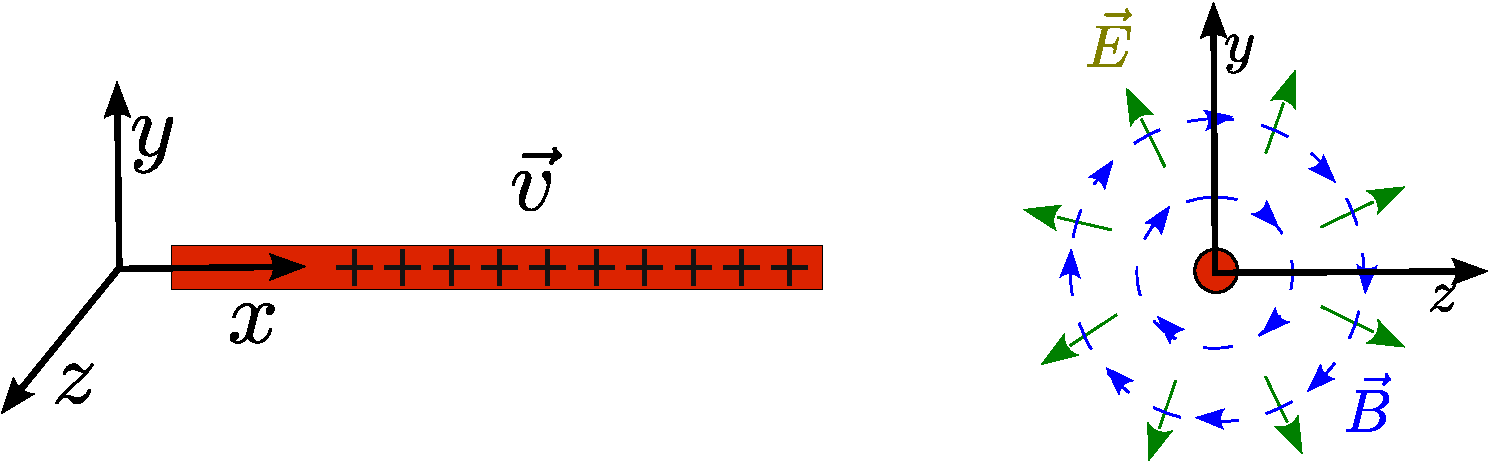
\psfig{file=fig-boost-campos-01.pdf,height=3.5cm,angle=0}}
\caption{Una l'inea de carga movi'endose con velocidad $v$ a lo largo de su eje.} \label{fig:bc01}
\end{figure}
\end{center}
En particular, en el SRI $K'$ com'ovil con las cargas $v'=0$ y la l'inea de carga tiene una densidad lineal $\lambda'$, entonces
\begin{equation}
 \vec{E}'=\frac{\lambda'}{2\pi\varepsilon_0}\left( \frac{y'\hat{y}+z'\hat{z}}{y'^2+z'^2}\right) , \qquad \vec{B}'=\vec{0}.
\end{equation}
En el SRI com'ovil $K'$ s'olo existe campo el'ectrico, que es normal a la direcci'on de la l'inea. Aplicamos ahora la transformaci'on de campos dada por (\ref{TLE}) y (\ref{TLE}). De acuerdo a esto, en el SRI donde la distribuci'on lineal de carga se mueve con velocidad $\vec{v}=v\hat{x}$, tendremos
\begin{equation}
 \vec{E}=\gamma\vec{E}'=\frac{\gamma\lambda'}{2\pi\varepsilon_0}\left( \frac{y\hat{y}+z\hat{z}}{y^2+z^2}\right) , \qquad \vec{B}= \frac{\gamma}{c^2}\vec{v}\times\vec{E}'=\frac{\gamma\lambda'}{2\pi\varepsilon_0c^2}\left( \frac{y\hat{z}-z\hat{y}}{y^2+z^2}\right). \label{clci2}
\end{equation}
Aqu'i hemos usado el hecho que bajo un boost a lo largo del eje $x$, $y'=y$ y $z'=z$. Vemos que (\ref{clci2}) coincide con (\ref{clci1}) luego de identificar $\lambda=\gamma\lambda'$, que es la relaci'on esperada entre las densidades lineales de carga, debido a la contracci'on relativista de longitudes a lo largo de la direcci'on de movimiento. Note que de las expresiones anteriores podemos escribir  $\vec{B}=\vec{v}\times\vec{E}/c^2$.

\subsubsection{Ejemplo 2}
Un ejemplo complementario lo suministra el caso de un magneto que genera, en su SRI com'ovil $K'$, un campo un campo magn'etico como el ilustrado en la figura. Aqu'i entonces $\vec{E}'=\vec{0}$ y $\vec{B}'\neq\vec{0}$. En un SRI donde el magneto se mueve con velocidad $v$ a lo largo del eje $x$ com'un existir'a, como consecuencia de la ley de Faraday, un campo el'ectrico inducido perpendicular a la direcci'on de movimiento. Las expresiones encontradas para la transformaci'on de los campos bajo un boost implican, en este caso,
\begin{equation}
 \vec{E}=-\gamma\left(\vec{v}\times\vec{B}'\right), \qquad
\vec{B}=\gamma \vec{B}'-\frac{(\gamma -1)}{v^2}\left( \vec{v}\cdot
\vec{B}'\right) \vec{v}.
\end{equation}
Verificamos, en particular, que el campo el'ectrico en este nuevo SRI es normal a la direcci'on de movimiento del magneto.

Adicionalmente, considere el caso en que se ubica una carga $q$ a una cierta distancia del magneto, con velocidad inicial nula respecto de 'el. Entonces, en el SRI com'ovil la carga tendr'a velocidad inicial nula y la fuerza total sobre ella ser'a tambi'en cero, ya que no existe campo el'ectrico en dicho SRI. En el SRI en el que el magneto se mueve con velocidad $\vec{v}$ la carga tendr'a una velocidad inicial igual a la del magneto ($\vec{v}$). De esta forma, la carga $q$ ``sentir'a'' un campo el'ectrico y uno magn'etico. No obstante, la fuerza total sobre ella es tambi'en nula:
\begin{eqnarray}
\vec{F}&=&q\left(\vec{E}+\vec{v}\times\vec{B}\right) \\
&=&q\left(-\gamma\,\vec{v}\times\vec{B}'+ \vec{v}\times\left[\gamma \vec{B}'-\frac{(\gamma -1)}{v^2}\left( \vec{v}\cdot
\vec{B}'\right) \vec{v}\right]\right)\\
&=&q\left(-\gamma\, \vec{v}\times\vec{B}'+\gamma\,\vec{v}\times\vec{B}'+0\right)\\
&=&\vec{0}.
\end{eqnarray}
Verificamos en este ejemplo que la descripci'on de la interacci'on entre el magneto y la carga es diferente en los dos SRI's discutidos, en un SRI s'olo hay presente un campo magn'etico. En el otro, debido a la ley de Faraday, se induce adem'as un campo el'ectrico. Ambas descripciones, sin embargo, conciden en su predicci'on final: la carga no alterar'a su estado de movimiento ya que la fuerza sobre ella es nula.


\subsubsection{Ejemplo 3: Campo generado por una carga movi'endose con velocidad constante}\label{secEjEBvc}
Aqu'i aplicaremos la ley de transformaci'on del campo electromagn'etico bajo
TL's para encontrar el campo producido por una carga movi'endose con velocidad constante respecto a un SRI $K$. Para ello, encontraremos primero los campos en el SRI $K'$ que es com'ovil con la carga y luego transformaremos estos campos al SRI $K$ usando la TL apropiada.

Elegimos los ejes de modo que la carga se mueva a lo largo del eje $x$ ($x'$ respecto a $K'$). En el SRI $K'$, un evento $P$, donde queremos determinar el campo electromagn'etico, tiene coordenadas $x'^\mu(P)=(ct',\vec{x}')$. Bajo estas condiciones, el campo electromagn'etico, que en $K'$ corresponde simplemente a un campo el'ectrost'atico coulombiano, adopta la forma:
\begin{equation}
\vec{E}'(P)=\frac{q}{4\pi\varepsilon_0}\frac{\vec{x}'}{r'^3}, \qquad \vec{B}' =\vec{0}. \label{EBp}
\end{equation}
Aplicando la ley de transformaci'on (\ref{TLE}) y (\ref{TLB}) (en realidad, la
\textit{inversa} de estas transformaciones, que equivalen a reemplazar
$\vec{\beta}$ por $-\vec{\beta}$) obtenemos que en $K$
\begin{equation}
\vec{E}=\gamma \vec{E}'-\frac{(\gamma -1)}{\beta^2}\left( \vec{\beta}\cdot
\vec{E}'\right) \vec{\beta} , \qquad
\vec{B}=\frac{\gamma}{c} \left(\vec{\beta}\times\vec{E}'\right).
\end{equation}
Usando (\ref{EBp}) podemos escribir los campos en funci'on de las coordenadas
$\vec{x}'$:
\begin{equation}
\vec{E}=\frac{q}{4\pi\varepsilon_0}\frac{\gamma \vec{x}'-\frac{(\gamma -1)}{\beta^2}(\vec{\beta}\cdot
\vec{x}')\vec{\beta}}{r'^3}  , \qquad
\vec{B}=\frac{q}{4\pi\varepsilon_0 c}\gamma \left(\vec{\beta}\times\frac{\vec{x}'}{r'^3}\right),
\end{equation}
Finalmente, usando la expresi'on de $\vec{x}'$ en funci'on de $\vec{x}$ y $t$
correspondiente, es decir, aquella dada en (\ref{bg1}), llegamos a
\begin{align}
\vec{E}(x) &= \frac{q}{4\pi\varepsilon_0}\frac{\gamma\left( \vec{x}-\vec{\beta}ct\right)}
{\left[\vec{x}^2+\gamma^2\left(\vec{\beta}\cdot\vec{x}-ct\right)^2-c^2t^2\right]^{3/2}} , \\
\vec{B}(x) &= \frac{q}{4\pi\varepsilon_0c}\frac{\gamma\left( \vec{\beta}\times\vec{x}\right) }
{\left[\vec{x}^2+\gamma^2\left(\vec{\beta}\cdot\vec{x}-ct\right)^2-c^2t^2\right]^{3/2}}.
\end{align}
Aqu'i hemos usado $\gamma \vec{x}'-(\gamma -1)(\vec{\beta}\cdot\vec{x}')\vec{\beta}/\beta^2=\gamma\left( \vec{x}-\vec{\beta}ct\right) $ y
$r'^2=\vec{x}'^2=\vec{x}^2+\gamma^2\left(\vec{\beta}\cdot\vec{x}-ct\right)^2-c^2t^2$, que se deducen directamente de (\ref{bg1}).

Si adem'as consideramos $\vec{\beta}=({v}/{c},0,0)$, donde $v$ es
la rapidez de la part'icula, entonces
\begin{eqnarray}
\vec{E}(x)&=&\frac{q}{4\pi\varepsilon_0}\frac{\gamma (\vec{x}-\vec{x}t)}{\left[\gamma^2 (x-vt)^2+y^2+z^2\right]^{3/2}} ,
\label{Evx}\\
\vec{B}(x)&=&\frac{q}{4\pi\varepsilon_0c^2}\frac{\gamma v \left(z\hat{y}-y\hat{z}\right)}{\left[\gamma^2 (x-vt)^2+y^2+z^2\right]^{3/2}}, \label{Bvx}
\end{eqnarray}
ya que $ x^2+\gamma^2(\beta x)^2=\gamma^2x^2$.

Este resultado coincide con aquel en el cap'itulo \ref{caprad}, obtenido resolviendo directamente las ecuaciones de Maxwell para una part'icula en movimiento rectil'ineo, ver \eqref{EBqvconst}.

%
% Las superficies de igual intensidad de campo no son esferas, sino elipsoides
% de revoluci'on en funci'on de $\theta$, ya que:
% \begin{equation}
% \left(  b^2+\gamma^2v^2t^2\right)  ^{3/2}=\left(
% r^2\operatorname{sen}^2\theta+\gamma^2r^2\cos^2\theta\right)^{3/2},
% \end{equation}
% y adem'as
% \begin{align}
% r^2\operatorname{sen}^2\theta+\gamma^2r^2\cos^2\theta &
% =r^2\left(  \operatorname{sen}^2\theta+\gamma^2\cos^2\theta\right) \\
% & =r^2\left(  \operatorname{sen}^2\theta+\gamma^2\left(
% 1-\operatorname{sen}^2\theta\right)  \right) \\
% & =r^2\left(  \operatorname{sen}^2\theta+\gamma^2-\gamma^2%
% \operatorname{sen}^2\theta\right) \\
% & =r^2\left(  \gamma^2+\left(  1-\gamma^2\right)  \operatorname{sen}%
%^2\theta\right) \\
% & =r^2\left(  \gamma^2-\gamma^2\beta^2\operatorname{sen}^2%
% \theta\right) \\
% & =r^2\gamma^2\left(  1-\beta^2\operatorname{sen}^2\theta\right) ,
% \end{align}
% de modo que
% \begin{equation}
% \left(  b^2+\gamma^2v^2t^2\right)  ^{3/2}=r^3\gamma^3\left(
% 1-\beta^2\operatorname{sen}^2\theta\right)  ^{3/2} .
% \end{equation}
% Reemplazando esto, obtenemos
% \begin{align}
% E_1  & =-\frac{q\gamma r\cos\theta}{r^3\gamma^3\left(  1-\beta
%^2\operatorname{sen}^2\theta\right)  ^{3/2}}=-\frac{qr\cos\theta}%
% {r^3\gamma^2\left(  1-\beta^2\operatorname{sen}^2\theta\right)
% ^{3/2}} ,\\
% E_2  & =\frac{q\gamma r\operatorname{sen}\theta}{r^3\gamma^3\left(
% 1-\beta^2\operatorname{sen}^2\theta\right)  ^{3/2}}=\frac
% {qr\operatorname{sen}\theta}{r^3\gamma^2\left(  1-\beta^2%
% \operatorname{sen}^2\theta\right)  ^{3/2}}.
% \end{align}
% Ahora bien, el vector que conecta la carga y el punto $P$ tiene componentes
% \begin{equation}
% r^1   =-r\cos\theta, \qquad r^2   =r\operatorname{sen}\theta
% \end{equation}
% y, por lo tanto,
% \begin{equation}
% E^i=\frac{qr^i}{r^3\gamma^2\left(  1-\beta^2\operatorname{sen}%
%^2\theta\right)  ^{3/2}}.
% \end{equation}
% Note que aunque el campo es radial, no es is'otropico. A lo largo
% de la direcci'on de movimiento, cuando $\theta=0$ 'o $\pi$, el campo es
% menor que cuando es $\pi/2$ 'o $-\pi/2$.


\subsection{Invariantes electromagn'eticos}

Si bien hemos visto que bajo un cambio de SRI (las componentes de) los campos
el'ectrico y magn'etico cambian su valor, existen ciertas combinaciones de ellos que permanecen inalterados, es decir, con el mismo valor, bajo una TL. Estas cantidades escalares \textit{pueden ser construidas a partir del tensor electromagn'etico} y los otros tensores disponibles, que en nuestro caso son la m'etrica $\eta$ y el s'imbolo de Levi-Civita (o, equivalentemente, el tensor dual $\cal F$).

Considere entonces los siguientes escalares\footnote{En rigor $I_2$, tal como lo definimos aqu'i es un \textit{pseudoescalar}. En este curso no haremos
distinci'on entre escalares y pseudoescalares.}:
\begin{align}
I_1 & :=\frac{1}{2}\eta^{\mu\lambda}\eta^{\nu\rho}F_{\mu\nu}F_{\lambda\rho}=\frac{1}{2}F_{\mu\nu}F^{\mu\nu},\\
I_2 & :=\frac{1}{4}\epsilon^{\mu\nu\lambda\rho}F_{\mu\nu}F_{\lambda\rho}
= \frac{1}{2}F_{\mu\nu}{\cal F}^{\mu\nu}.
\end{align}
Usando (\ref{Fdndn}), (\ref{Fupup}) y (\ref{Fdualupup}) podemos reescribir los invariantes $I_1$ y $I_2$ en funci'on de $\vec{E}$ y $\vec{B}$:
\begin{equation}
I_1=\vec{B}^2-\frac{1}{c^2}\vec{E}^2, \qquad I_2  =-\frac{2}{c}\vec{E}\cdot\vec{B}.
\end{equation}

El hecho que $I_1$ e $I_2$ permanezcan invariantes bajo TL's puede usarse para
obtener diversos resultados, tales como:
\begin{itemize}
\item Si en un SRI $\vec{E}^2<c^2\vec{B}^2$, entonces \textit{no es posible
encontrar un SRI en el que} $\vec{B}=\vec{0}$.
\item Si en un SRI $c^2\vec{B}^2<\vec{E}^2$, entonces \textit{no es posible
encontrar un SRI en el que} $\vec{E}=\vec{0}$.
\item Si en un SRI $\vec{E}$ es perpendicular a $\vec{B}$, entonces $\vec{E}$
ser'a perpendicular a $\vec{B}$ \textit{en todo SRI}.
\item Si en un SRI $\vec{E}\cdot\vec{B}\neq 0$, entonces \textit{no es posible encontrar un SRI en el que} $\vec{E}=\vec{0}$ o $\vec{B}=\vec{0}$.
\end{itemize}
Note que las afirmaciones anteriores son v'alidas para los valores de $\vec{E}$
y $\vec{B}$ \textit{en un evento} dado. En general, si ninguno de los criterios anteriores lo impide, es posible encontrar un SRI que cumpla con alg'una condici'on requerida. Por ejemplo, si en un SRI $\vec{E}^2<c^2\vec{B}^2$ y $\vec{E}\cdot\vec{B}=0$, entonces es posible encontrar un SRI en el que $\vec{E}=\vec{0}$.


\section{Potenciales y transformaciones de gauge}

El potencial escalar $\phi$ y el potencial vectorial $\vec{A}$ (en cojunto ``los potenciales electromagn'eticos'') son campos definidos de forma tal que los campos el'ectrico y magn'etico satisfagan autom'aticamente las ecuaciones de Maxwell homog'eneas: 
\begin{equation}\label{defphi}
\vec{E} =  - \frac{\partial \vec{A}}{\partial t} - \vec{\nabla}\phi ,
\end{equation}
\begin{equation}\label{BrotA}
\vec{B}=\vec{\nabla}\times \vec{A}.
\end{equation}
Los potenciales no son funciones definidas un'ivocamente dada una configuraci'on de campo electromag'etico. Esto se manifiesta en la invariancia de los campos $\vec{E}$ y $\vec{B}$ bajo una transformaci'on de gauge:
\begin{equation}
\phi' =\phi +\frac{\partial \chi}{\partial t}, \qquad
{\vec{A}}' = \vec{A} - \vec{\nabla}{\chi},
\end{equation}
donde $\chi=\chi(\vec{x},t)$ es una funci\'on \textit{arbitraria} del espaciotiempo

En la formulaci'on relativista, los potenciales electromagn'eticos son componentes de un  \textit{4-potencial electromagn'etico} (o, simplemente 4-potencial), definido por
\begin{equation}
A^\mu =(\phi/c,\vec{A}), \qquad A_\mu =(\phi/c,-\vec{A}). \label{identA}
\end{equation}
En t'erminos de este 4-potencial, las expresiones (\ref{defphi}) y (\ref{BrotA}) se condensan en
\begin{equation}
\boxed{F_{\mu \nu}=\partial_\mu A_{\nu}-\partial_{\nu}A_\mu.} \label{fda}
\end{equation}

Ya que $F_{\mu\nu}$ es un tensor tipo $(0,2)$, para que la relaci'on (\ref{fda})
se v'alida en todo SRI es necesario que $A_\mu$ constituya un vector
\textit{covariante} bajo TL's.

Una transformaci\'on de gauge adopta entonces la forma
\begin{equation}
\boxed{A_\mu' = A_\mu  + \partial_\mu  \chi .}
\end{equation}
Bajo esta transformaci'on, el tensor electromagn'etico $F_{\mu \nu}$ permanece
invariante. En efecto,
\begin{eqnarray}
F_{\mu\nu}'&=&\partial_\mu A_{\nu}'-\partial_{\nu}A_\mu '  \\
&=&\partial_\mu (A_{\nu}+\partial_{\nu}
\chi)-\partial_{\nu}(A_\mu +\partial_\mu  \chi)\\
&=&\partial_\mu A_{\nu}-\partial_{\nu}A_\mu  \\
&=&F_{\mu \nu}.
\end{eqnarray}

\subsection{Gauge de Lorenz}
Es directo escribir la condici'on de Lorenz en forma covariante. Usando
(\ref{identA}) obtenemos que
\begin{equation}
\frac{1}{c^2}\frac{\partial\phi}{\partial t}+\vec{\nabla}\cdot\vec{A}=0,
\end{equation}
es equivalente a
\begin{equation}
\partial_\mu A^\mu=0. \label{gLA}
\end{equation}
Ya que el 4-potencial es un vector bajo TL's, vemos que la condici'on que define el gauge de Lorenz es una ecuaci'on covariante (en particular, es una \textit{ecuaci'on escalar}). Esto asegura que si el gauge de Lorenz se satisface en un SRI $K$ con los potenciales $\phi$ y $\vec{A}$ correspondientes, entonces ser'a tambi'en satisfecho en todo SRI $K'$, con los potenciales $\phi'$ y $\vec{A}'$ transformados. Esta propiedad hace que el gauge de Lorenz sea ampliamente usado en el contexto de la teor'ia de relatividad especial, puesto que permite trabajar con los potenciales electromagn'eticos, simplificar muchas ecuaciones al imponer el gauge de Lorenz, pero de forma tal que los resultados sean v'alidos en cualquier SRI. Esta 'util propiedad no es v'alida, por ejemplo, usando el gauge de Coulomb.

Si el 4-potencial satisface el gauge de Lorenz, la ecuaci'on diferencial que 'este debe satisfacer se reduce a la \textit{ecuaci'on de onda inhomogenea}
\begin{equation}
\boxed{\square A^\mu=\mu_0 J^\mu .} \label{caj}
\end{equation}

En efecto, escribiendo las ecuaciones de Maxwell inhomogeneas (\ref{emihF}) en t'erminos del 4-potencial, encontramos que
\begin{align}
\mu_0 J^\nu &=\partial_\mu F^{\mu\nu}  \\
&=\partial_\mu \left(  \partial^\mu A^\nu -\partial^\nu A^\mu \right)  \\
&= \partial_\mu \partial^\mu A^\nu -\partial_\mu \partial^\nu A^\mu   \\
&= \square A^\nu -\partial^\nu (\partial_\mu A^\mu)   ,
\end{align}
que se reduce a (\ref{caj}) cuando $A_\mu$ satisface (\ref{gLA}).

\section{Forma covariante de la Fuerza de Lorentz}
Sabemos que en mec'anica no-relativista la fuerza de Lorentz, que describe c'omo el campo electromagn'etico act'ua sobre cargas de prueba, es de la forma
\begin{equation}
\frac{d\vec{p}}{dt}=q\left(  \vec{E}+\vec{v}\times\vec{B}\right).
\label{dpdt}
\end{equation}
Sabemos que en RE el mom'entum est'a contenido en el 4-mom'entum, junto con la
energ'ia de la part'icula. Por tanto, la ecuaci'on anterior debe ser
complementada con la ecuaci'on que expresa la variaci'on de la energ'ia de la
part'icula en funci'on del tiempo. Es conocido en mec'anica no-relativista que
la potencia (trabajo por unidad de tiempo) realizada por el campo
electromagn'etico sobre una carga es $q\,\vec{v}\cdot\vec{E}$, de modo que
\begin{equation}
\frac{dE}{dt}=q\,\vec{v}\cdot\vec{E}. \label{dEdt}
\end{equation}
Tomando en cuenta que energ'ia y mom'entum forman el vector de 4-mom'entum $p^\mu=({E}/{c},\vec{p})$ en RE, vemos que los lados
izquierdos de (\ref{dpdt}) y (\ref{dEdt}) corresponden a las componentes de
${dp^\mu}/{dt}$, mientras que los lados derechos son \textit{lineales en los campos y en la velocidad} (excepto $q\vec{E}$).

Consideremos entonces una expresi'on tensorial, lineal en el tensor
electromagn'etico y en la 4-velocidad, a saber: $F^\mu{}_{\nu}u^\nu$. Las
componentes temporales y espaciales de este 4-vector son
\begin{eqnarray}
F^0{}_{\nu}u^\nu &=&F^0{}_{i}u^i=\frac{\gamma}{c}\vec{E}\cdot\vec{v} ,\\
F^i{}_{\nu}u^\nu &=&F^i{}_{0}u^0+F^i{}_{j}u^j=\gamma \left(
E^i+\epsilon^{ijk}B^j v^k\right) .
\end{eqnarray}
Con esto, podemos escribir  (\ref{dpdt}) y (\ref{dEdt}), sin modificaci'on
alguna, como
\begin{equation}
\frac{dp^\mu }{dt}=\frac{q}{\gamma}F^\mu _{\ \ \nu}u^\nu ,
\end{equation}
o, en \textit{t'erminos del tiempo propio de la part'icula} ($dt=\gamma d\tau$),
finalmente como
\begin{equation}
\boxed{\frac{dp^\mu }{d\tau}=qF^\mu _{\ \ \nu}u^\nu .} \label{LorRel}
\end{equation}
En resumen, es posible escribir la ecuaci'on de fuerza de Lorentz en forma
covariante (lo que asegura su validez en todo SRI), \textit{sin necesidad de
modificarla expl'icitamente}. Note, sin embargo que, debido a que la energ'ia y el mom'entum relativista tienen expresiones distintas a aquellas usadas en mec'anica no-relativista (y por tanto, asumen valores distintos para la mismas masas y velocidades), las \textit{trayectorias} \textit{predichas}\footnote{o `modeladas', o `descritas' \dots} \textit{por (\ref{LorRel}) ser'an distintas} a aquellas determinadas en la mec'anica no-relativista (para una carga y campos dados).

\subsection{Ejemplo}
Considere el caso de una part'icula de carga $q$ en una regi'on del espacio(tiempo) donde s'olo existe un campo el'ectrico uniforme. Orientaremos los ejes espaciales de modo que el campo el'ectrico s'olo tenga componente a lo largo del eje $x$ positivo, es decir, $\vec{E}=(E,0,0)$ y adem'as $\vec{B}=\vec{0}$. Con esto, el movimiento de la part'icula ser'a unidimensional. Asumiremos adem'as las condiciones iniciales $\vec{x}(0)=\vec{0}$ y $\vec{v}(0)=\vec{0}$, y nos proponemos
encontrar la trayectoria que describe esta part'icula de acuerdo a las
ecuaciones de movimiento no-relativistas y relativistas.

\subsubsection{Modelo no-relativista:}

En este caso, la ecuaci'on de movimiento que determina la trayectoria de la
part'icula es
\begin{equation}
m\frac{d^2x}{dt^2}=qE,
\end{equation}
cuya soluci'on es
\begin{equation}
x(t)=\frac{qE}{2m}t^2, \qquad v(t)=\frac{qE}{m}t.
\end{equation}
Esta soluci'on, tal como se espera en el contexto de la mec'anica
no-relativista, permite en principio que la velocidad de la part'icula aumente
indefinidamente.

\subsubsection{Modelo relativista:}

De acuerdo a (\ref{LorRel}), y recordando la definici'on del 4-mom'entum (\ref{def4mom}), tenemos que en este caso las ecuaciones de movimiento relativistas adoptan la forma
\begin{eqnarray}
\frac{du^0}{d\tau}&=& \frac{qE}{mc} u^1, \label{mre1} \\
\frac{du^1}{d\tau}&=&\frac{qE}{mc} u^0.\label{mre2}
\end{eqnarray}
Derivando (\ref{mre1}) y reeemplazando en (\ref{mre1}) obtenemos
\begin{equation}
 \frac{d^2u^0}{d\tau^2}=\left( \frac{qE}{mc}\right)^2 u^0,
\end{equation}
cuya soluci'on es de la forma
\begin{equation}
u^0(\tau)=A\senh\left( \frac{qE}{mc}\tau\right)+B\cosh\left(
\frac{qE}{mc}\tau\right). \label{mrsu0}
\end{equation}
Reemplazando esta soluci'on en (\ref{mre1}) encontramos adem'as que
\begin{equation}
u^1(\tau)=A\cosh\left( \frac{qE}{mc}\tau\right)+B\senh\left(
\frac{qE}{mc}\tau\right). \label{mrsu1}
\end{equation}
Integrando (\ref{mrsu0}) y (\ref{mrsu1}) encontramos la soluci'on para las coordenadas en t'erminos del tiempo propio,
\begin{eqnarray}
x^0(\tau)&=&\left(\frac{mc}{qE}\right)\left[A\cosh\left( \frac{qE}{mc}\tau\right)+B\senh\left(
\frac{qE}{mc}\tau\right)+\alpha\right] ,\\
x^1(\tau)&=&\left(\frac{mc}{qE}\right)\left[A\senh\left( \frac{qE}{mc}\tau\right)+B\cosh\left(
\frac{qE}{mc}\tau\right)+\alpha'\right] .
\end{eqnarray}
Debemos a'un determinar las constantes $A$, $B$, $\alpha$ y $\alpha'$. Para esto, imponemos las condiciones iniciales $x^0(0)=0$, $x^1(0)=0$ y $\vec{v}_0=\vec{0}$, que en nuestro caso es equivalente a $u^1(0)=0$. Estas condiciones requieren que $\alpha=-A$ y $\alpha'=-B$ y adem'as $A=0$. Con esto, la soluci'on se reduce a
\begin{eqnarray}
x^0(\tau)&=&\left(\frac{mc}{qE}\right)B\senh\left(\frac{qE}{mc}\tau\right) ,\\
x^1(\tau)&=&\left(\frac{mc}{qE}\right)B\left[\cosh\left(
\frac{qE}{mc}\tau\right)-1\right] .
\end{eqnarray}
Podemos determinar la constante $B$ de la condici'on $u^\mu
u_\mu=(u^0)^2-(u^1)^2=c^2$. As'i obtenemos $B=c$, de modo que la
soluci'on de las ecuaciones de movimiento relativistas para nuestro ejemplo es:
\begin{eqnarray}
ct(\tau)&=&\frac{mc^2}{qE}\senh\left( \frac{qE}{mc}\tau\right), \label{cttau}\\
x(\tau)&=&\frac{mc^2}{qE}\left[ \cosh\left( \frac{qE}{mc}\tau\right)-1\right] .
\end{eqnarray}

Finalmente, podemos expresar la posici'on $x$ en funci'on del tiempo $t$,
despejando $\tau$ en funci'on de $t$ de (\ref{cttau}). As'i obtenemos:
\begin{equation}
x(t) = \frac{mc^2}{qE} \left[ \sqrt{1 + \frac{q^2 E^2 t^2}{m^2c^2}} - 1 \right].
\label{xtsol}
\end{equation}
La correspondiente velocidad es entonces
\begin{equation}
v(t) = \frac{qE}{m}\frac{t}{\sqrt{1 + \frac{q^2 E^2 t^2}{m^2c^2}}}.
\end{equation}
Verificamos que para tiempos ``peque\~nos'', $t\ll {mc}/{qE}$, la soluci'on se
reduce a aquella encontrada en el contexto no-relativista. Sin embargo, la
soluci'on (\ref{xtsol}) difiere de la no-relativista para tiempos grandes
comparados con ${mc}/{qE}$, en los que la carga alcanza velocidades
relativistas ($v={c}/{\sqrt{2}}\approx 0,7c$ para $t={mc}/{qE}$). Como esperamos, la soluci'on relativista asegura que la velocidad de la part'icula es siempre subluminal.

\begin{center}
\begin{figure}[H]
\centerline{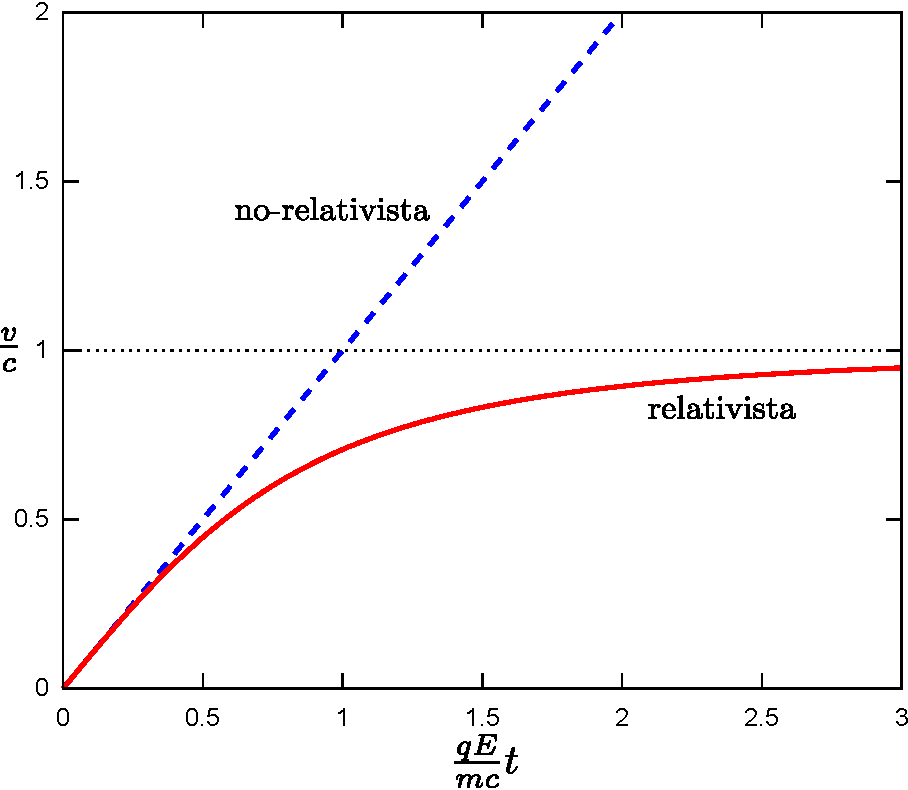
\psfig{file=fig-trayectoria-1D-rel-norel.pdf,height=7cm,angle=0}}
\caption{Comparaci'on entre velocidades seg'un ecuaci'on de Lorentz relativista y no-relativista.}
\label{fig:relnorel}
\end{figure}
\end{center}


\subsubsection{F'ormula de Larmor relativista*}


Consideraremos nuevamente la expresi'on para la potencia radiada por una carga acelerada, pero ahora en el caso en que su velocidad no es despreciable comparada con la velocidad de la luz. El m'etodo directo para calcular la
potencia total radiada es rehacer el c'alculo de la secci'on \ref{sec:Larmor-norel}, pero usando el campo $\vec{E}_{(2)}$ general dado en (\ref{Egen}). Una forma alternativa es generalizar el resultado no-relativista teniendo en cuenta que \textit{la potencia es un escalar bajo TL's}. Esta propiedad de $P$ puede ser inferida considerando que la energ'ia irradiada en un intervalo de tiempo $dt$ es $dE=P(t)dt$, y el hecho que tanto la energ'ia ($dE$) y el tiempo ($dt$) transforman bajo TL's como las componentes temporales de un 4-vector (4-mom'entum y 4-posici'on, respectivamente). Usando ahora el hecho que $P$ es un invariante bajo TL's, podemos buscar una generalizaci'on de \eqref{R-larmor} que incluya la 4-aceleraci'on $\mathsf{a}^\mu$ en lugar de la aceleraci'on $\vec{a}$, que se reduzca en el l'imite no-relativista a \eqref{R-larmor} y que sea un escalar. La expresi'on apropiada que cumple estos requisitos es:
\begin{equation}
\boxed{P=-\frac{q^2\mu}{6\pi c}\,\mathsf{a}^\mu\mathsf{a}_\mu.}\label{R-larmor-rel}%
\end{equation}
Usando (\ref{4a2}) podemos escribir la potencia en el caso
relativista en t'erminos de la velocidad y aceleraci'on de la carga:
\begin{equation}
\boxed{P=\frac{q^2\mu}{6\pi c}\,\gamma^6\left[ \vec{a}^2-\left(\vec{\beta}\times\vec{a}\right)^2\right] .}\label{R-larmor2}%
\end{equation}
Note que, tanto en el caso relativista como no-relativista, si las cargas son
aceleradas por una misma fuerza (por ejemplo por un campo el'ectrico externo)
entonces las cargas de menor masa irradiar'an m'as energ'ia que las m'as
masivas, ya que su aceleraci'on ser'a mayor. Por ejemplo, en un plasma con
electrones y protones acelerados por un campo el'ectrico externo, la potencia
radiada por los electrones ser'a aproximadamente $(1836)^2\approx 3\times
10^{6}$ veces mayor que aquella radiada por los protones, ya que $m_p\approx
1836\,m_e$.

En general, podemos escribir
\begin{equation}
\mathsf{a}^\mu\mathsf{a}_\mu=\frac{1}{m^2}\frac{dp^\mu}{d\tau}\frac{dp_\mu}{
d\tau}=\frac{1}{m^2c^2}\left( \frac{dE}{d\tau}\right)^2-\frac{1}{m^2}\left(
\frac{d\vec{p}}{d\tau}\right)^2.
\end{equation}
Por otro lado, derivando la relaci'on $E^2=\vec{p}^2c^2+m^2c^4$, obtenemos
\begin{equation}
\frac{dE}{d\tau}=c^2\frac{p}{E}\frac{dp}{d\tau}=v\frac{dp}{d\tau},
\label{dEdtau}
\end{equation}
donde $p$ es el m'odulo del mom'entum $\vec{p}$. Usando (\ref{dEdtau}) podemos
reescribir (\ref{R-larmor-rel}) como
\begin{equation}
P=-\frac{q^2\mu}{6\pi m^2c}\left[ \beta^2\left(
\frac{dp}{d\tau}\right)^2-\left( \frac{d\vec{p}}{d\tau}\right)^2\right] .
\label{4a2-2}
\end{equation}

\subsubsection{Ejemplo: Aceleradores lineales}
Consideramos ahora el caso particular de un movimiento unidimensional. En este
caso $\vec{p}=p\hat{p}$ donde $\hat{p}$ es constante, de modo que
${d\vec{p}}/{d\tau}=({dp}/{d\tau})\hat{p}$ y entonces
\begin{eqnarray}
\beta^2\left(\frac{dp}{d\tau}\right)^2-\left( \frac{dp}{d\tau}\right)^2
&=&\left( \beta^2-1\right) \left(  \frac{dp}{d\tau}\right)^2\\
&=&-\frac{1}{\gamma^2} \left(  \frac{dp}{d\tau}\right)^2\\
&=&-\left(\frac{dp}{dt}\right)^2.
\end{eqnarray}
Aqu'i usamos el hecho que $dt=\gamma d\tau$. Con esto podemos escribir la f'ormula de Larmor relativista (\ref{4a2-2}) para el caso de movimiento unidimensional como:
\begin{equation}
\boxed{P_{1d}=\frac{q^2\mu}{6\pi m^2c}\left(  \frac{dp}{dt}\right)^2.}
\end{equation}
Alternativamente, introduciendo la \textit{tasa de cambio de la energ'ia de la
carga por unidad de longitud recorrida}
\begin{equation}
 \frac{dE}{dl}=\frac{\frac{dE}{dt}}{\frac{dl}{dt}}=\frac{1}{v}\frac{dE}{dt}
= \frac{dp}{dt},
\end{equation}
encontramos
\begin{equation}
\boxed{P_{1d}=\frac{q^2\mu}{6\pi m^2c}\left(  \frac{dE}{dl}\right)^2.}% aqui cambie
\end{equation}
Se acostumbra definir la fracci'on de potencia radiada respecto a la energ'ia
suministrada a la part'icula por unidad de tiempo:
\begin{equation}
\eta:=\frac{\left( \text{Potencia radiada}\right) }{\text{(Potencia entregada a la carga)}}=\frac{P}{\frac{dE}{dt}}.
\end{equation}
Usando los resultados anteriores encontramos que
\begin{equation}
\eta=\frac{q^2\mu}{6\pi m^2c}\frac{1}{v}\frac{dE}{dl}.
\end{equation}
En el caso ultra-relativista $v\approx c$ (como en los aceleradores de
part'iculas), tenemos que
\begin{equation}
\eta\approx\frac{q^2\mu}{6\pi m^2c^2}\frac{dE}{dl}.
\end{equation}
En el caso de los aceleradores lineales se est'a interesado en minimizar las
``p'erdidas'' de energ'ia por radiaci'on, es decir, se requiere que $\eta\ll 1$.
Esto ocurre si las cargas son aceleradas ``lentamente'' de modo que
\begin{equation}
\frac{dE}{dl}\ll \frac{6\pi m^2c^2}{q^2\mu}.
\end{equation}
Para electrones encontramos que ${6\pi m^2c^2}/{q^2\mu}\approx 2\times 10^4\, 
[MeV/m]$. Esta condici'on es satisfecha, por ejemplo, en un acelerador lineal como
el SLAC\footnote{\url{http://www.slac.stanford.edu}.}, donde se consigue
${dE}/{dl}\approx 50\, [MeV/m]$.

\section{Formalismo Lagrangeano*}
\subsection{La acci'on para una part'icula.}
Nos basaremos en el \emph{principio de m'inima acci'on}, o
principio de Hamilton. El principio de m'inima acci'on
establece que un sistema mec'anico es tal que al ir desde una
configuraci'on en el instante $t_1$ hasta otra configuraci'on en el instante
$t_2$, la \textit{acci'on} $S$,
\begin{equation}
S=\int L\left[  q^i(t),\dot{q}^i(t)  ,t\right]  dt, \label{Sdt}
\end{equation}
\textit{adopta un valor extremo}.

La acci'on tiene unidades $\left[  S\right]  = \text{[Energ'ia][Tiempo]=[Mom'entum][Distancia]}=[\hbar]=ML^2T^{-1}$.

Al considerarse variaciones peque\~nas de las coordenadas y
velocidades, la condici'on de extremo de $S$, $\delta S=0$, implica las
ecuaciones de movimiento de \textit{Euler-Lagrange}:
\begin{equation}
\frac{d}{dt}\left(  \frac{\partial L}{\partial\dot{q}^i}\right)
-\frac{\partial L}{\partial q^i}=0.\label{L-euler}%
\end{equation}

Requerimos que $S$ sea un escalar bajo TL's. Esto asegura que las ecuaciones de
movimiento ser'an covariantes bajo TL's, respetando as'i el principio de
relatividad. Usando $dt=\gamma d\tau$, encontramos que $S$ ser'a escalar si
$L':=L\gamma$ es escalar, de modo que
\begin{equation}
S=\int L' d\tau.
\end{equation}
Por lo tanto, necesitamos encontrar un escalar $L'=L'(x^\mu,u^\mu)$. Esperamos
adem'as que $L'$ no dependa expl'icitamente de las coordenadas $x^\mu$,
respetando as'i la invariancia bajo translaciones asumida en RE. El escalar $m u^\mu u_\mu$  es an'alogo a $m\vec{v}^2$  que, salvo factores
num'ericos, es el lagrangeano no-relativista de una part'icula libre de masa $m$. Sin embargo, en RE $m u^\mu u_\mu\equiv mc^2$, es decir, una constante. Esto podr'ia sugerir considerar $L'$ proporcional a la constante $mc^2$. Definamos entonces,
\begin{equation}
L'=\alpha mc^2,
\end{equation}
donde hemos introducido la constante adimensional $\alpha$, y veamos si la acci'on resultante conduce a las ecuaciones de movimiento correctas para una part'icula libre.

En este caso, tenemos
\begin{equation}
S=\alpha mc^2\int  d\tau=\alpha mc^2\int \frac{1}{\gamma}dt=\alpha mc^2\int
\sqrt{1-\frac{v^2}{c^2}}\,dt=\int L dt, \label{lagrellibre0}
\end{equation}
con $L=\alpha mc^2 \sqrt{1-\frac{v^2}{c^2}}$.
Para velocidades no-relativistas $\sqrt{1-\frac{v^2}{c^2}}=1-\frac{v^2}{2c^2}+O(\frac{v^4}{c^4})$  de modo que
\begin{equation}
L=\alpha mc^2-\frac{\alpha}{2}mv^2+O(\frac{v^4}{c^4}). \label{cL1}
\end{equation}
El primer t'ermino en el lado derecho de (\ref{cL1}) es irrelevante para nuestros fines puesto que no aporta a las ecuaciones de movimiento (es una derivada total). El segundo t'ermino ser'a igual al lagrangiano no-relativista de una part'icula libre si elegimos $\alpha=-1$. Con esta elecci'on aseguramos que en el l'imite no-relativista las ecuaciones de movimiento ser'an las apropiadas. Para velocidades arbitrarias, nuestro candidato a Lagrangiano para una part'icula relativista es
\begin{equation}
L=-mc^2 \sqrt{1-\frac{v^2}{c^2}},\label{lagrellibre}
\end{equation}
y la acci'on correspondiente,
\begin{equation}
\boxed{S=- mc^2\int  d\tau=\int L\, dt.}
\end{equation}

Considerando las variables de configuraci'on como $q^i=x^i(t)$, el lagrangiano (\ref{lagrellibre}) s'olo depende de las velocidades $\dot{q}^i=\dot{x}^i(t)$, por lo que los momenta can'onicos\footnote{El primero en introducir este mom'entum relativista fue Max Planck en 1906, usando el formalismo hamiltoniano, ver \cite{Planck06}.}
\begin{equation}
\frac{\partial L}{\partial \dot{x}^i}=\frac{mv^i}{\sqrt{1-\frac{v^2}{c^2}}}=p^i,
\end{equation}
son conservados. En efecto, las ecuaciones de movimiento son en este caso
\begin{equation}
\frac{d\ }{dt}\frac{\partial L}{\partial \dot{x}^i}-\frac{\partial L}{\partial x^i}=\frac{d p^i}{dt} =0,
\end{equation}
que es la ecuaci'on de movimiento correcta para una part'icula relativista
libre.

\subsubsection{Derivaci'on covariante*}

Podemos adem'as encontrar la ecuaci'on de movimiento en una forma expl'icitamente
covariante bajo TL's. Para esto introducimos un par'ametro admisible $\lambda$
sobre la trayectoria de la part'icula, y consideraremos como variables de
configuraci'on a $x^\mu(\lambda)$. En este caso, podemos escribir $S$ como
\begin{equation}
S=-mc^2\int  d\tau=-mc\int  ds=-mc\int  \frac{ds}{d\lambda}d\lambda=-mc\int
\sqrt{\eta_{\mu\nu}\frac{dx^\mu}{d\lambda}\frac{dx^\nu}{d\lambda}}\,
d\lambda=:\int  \tilde{L}\,d\lambda,
\end{equation}
con
\begin{equation}
\tilde{L}:=-mc\sqrt{\eta_{\mu\nu}\frac{dx^\mu}{d\lambda}\frac{dx^\nu}{d\lambda}}
. \label{Ltilde}
\end{equation}
De esta forma, describimos el sistema por un principio variacional an'alogo a
(\ref{Sdt}), donde $\tilde{L}$ reemplaza a $L$ y $\lambda$ a $t$. Debido a esto,
las ecuaciones de Euler-Lagrange en este caso son de la forma
\begin{equation}
\frac{d}{d\lambda}\left(  \frac{\partial
\tilde{L}}{\partial\left(\frac{dx^\mu}{d\lambda}\right) }\right)-\frac{\partial
\tilde{L}}{\partial x^\mu}=0.
\end{equation}
Usando (\ref{Ltilde}) encontramos que
\begin{equation}
 \frac{\partial \tilde{L}}{\partial\left(\frac{dx^\mu}{d\lambda}\right)
}=-\frac{mc}{\sqrt{\eta_{\mu\nu}\frac{dx^\mu}{d\lambda}\frac{dx^\nu}{d\lambda}}}
\,\eta_{\mu\nu}\frac{dx^\nu}{d\lambda}.
\end{equation}
Adem'as, como
\begin{equation}
\sqrt{\eta_{\mu\nu}\frac{dx^\mu}{d\lambda}\frac{dx^\nu}{d\lambda}}=\frac{ds}{
d\lambda}=c\frac{d\tau}{d\lambda},
\end{equation}
podemos escribir
\begin{equation}
 \frac{\partial \tilde{L}}{\partial\left(\frac{dx^\mu}{d\lambda}\right)
}=-m\,\eta_{\mu\nu}\frac{dx^\nu}{d\lambda}\frac{d\lambda}{d\tau}=-m\,\eta_{
\mu\nu}\frac{dx^\nu}{d\tau}=-m\,\eta_{\mu\nu}u^\mu=-\eta_{\mu\nu}p^\mu=-p_\mu.
\end{equation}
Por otro lado, ${\partial \tilde{L}}/{\partial x^\mu}=0$, de modo que las
ecuaciones de movimiento son
\begin{equation}
\frac{d}{d\lambda}p_\mu=0,
\end{equation}
o, equivalentemente
\begin{equation}
\frac{dp^\mu}{d\tau}  =0.
\end{equation}

\subsection{Part'icula en un campo electromagn'etico externo}

Ahora buscaremos la acci'on que describe la din'amica de una part'icula cargada
que se mueve en un campo electromagn'etico externo dado. Para esto, recordamos
que en el l'imite no-relativista, una carga $q$ en un potencial electrost'atico
$\phi$ tiene una energ'ia potencial de interacci'on $V=q\phi$. Como el
lagrangeano no-relativista es $T-V$, entonces la acci'on de interacci'on $S_\text{int, no-rel}$ es de la forma
\begin{equation}
S_\text{int, no-rel}= -q\int \phi\, dt. \label{L-rela02}%
\end{equation}
Consideramos ahora las posibles generalizaciones de (\ref{L-rela02}) al caso
relativista. Nuevamente, requerimos que la acci'on que describe la interacci'on
de la carga con el campo $S_{\rm int}$ (que se suma a la acci'on libre
(\ref{lagrellibre})) debe ser un escalar bajo TL's y reducirse a
(\ref{L-rela02}) para velocidades peque\~nas respecto a la de la luz.

Una acci'on que cumple con estos requisitos es
\begin{equation}
\boxed{S_{\rm int}=-q\int_{\tau_1}^{\tau_2}A_\mu u^\mu d\tau.}
\label{Sint}
\end{equation}
En efecto, escribiendo (\ref{Sint}) en t'erminos de las componentes espaciales y
temporales, encontramos que
\begin{equation}
S_{\rm int}=-q\int\left(  \phi u^0+A_i u^i\right)
d\tau=-q\int \left(\frac{1}{c}\phi \gamma c-\vec{A}\cdot\vec{v}\gamma \right)
\frac{1}{\gamma}dt =\int \left(-q\phi+q\vec{A}\cdot\vec{v}\right) dt ,
\label{L-rela03b}%
\end{equation}
que coincide con (\ref{L-rela02}) en el caso no-relativista (y/o
electrost'atico).

Consideramos ahora la acci'on completa para una part'icula de carga $q$, masa
$m$ en un campo electromagn'etico:
\begin{equation}
\boxed{S=-\int \left(mc^2+ qA_\mu u^\mu \right) d\tau.}
\end{equation}
Derivaremos las ecuaciones de movimiento en forma covariante usando nuevamente
el par'ametro $\lambda$ para parametrizar la trayectoria $x^\mu(\lambda)$ de la
part'icula en el espaciotiempo. En este caso $S=\int \tilde{L}d\lambda$ con
\begin{equation}
\tilde{L}:=-mc\sqrt{\eta_{\mu\nu}\frac{dx^\mu}{d\lambda}\frac{dx^\nu}{d\lambda}}-qA_\mu \frac{dx^\mu}{d\lambda}. \label{Ltilde2}
\end{equation}
Extendiendo el caso antes visto, tenemos que
\begin{equation}
 \frac{\partial\tilde{L}}{\partial\left(\frac{dx^\mu}{d\lambda}\right)}=-p_\mu-qA_\mu.
\end{equation}
Adem'as,
\begin{equation}
\frac{\partial \tilde{L}}{\partial x^\mu}=q\left( \partial_\mu
A_\nu\right)  \frac{dx^\nu}{d\lambda}.
\end{equation}
Con esto, las ecuaciones de movimiento son
\begin{equation}
\frac{d}{d\lambda}\left( -p_\mu -qA_\mu\right) -q\left(
\partial_\mu A_\nu\right)=0. \label{casicasi}
\end{equation}
Considerando que ${dA_\mu}/{d\lambda}=\left( \partial_\nu A_\mu \right)
({dx^\nu}/{d\lambda})$, podemos expresar (\ref{casicasi}) como
\begin{equation}
\frac{dp_\mu}{d\lambda} =q\left( \partial_\mu A_\nu-\partial_\nu
A_\mu\right)\frac{dx^\nu}{d\lambda}.
\end{equation}
Retornando a la parametrizaci'on en t'erminos del tiempo propio, encontramos que
la ecuaci'on de movimiento es
\begin{equation}
\frac{dp_\mu}{d\tau} =q\left( \partial_\mu A_\nu-\partial_\nu
A_\mu\right)u^\nu,
\end{equation}
que es exactamente la ecuaci'on de movimiento determinada por la fuerza de
Lorentz (\ref{LorRel}), ver ecuaci'on (\ref{fda}).


\subsection{Formalismo Lagrangeano para sistemas continuos (campos)}
Resumiremos aqu'i los aspectos b'asicos del formalismo lagrangeano para sistemas
con un continuo de grados de libertad (campos).

 Consideremos una \textit{densidad lagrangeana} que depende de $N$ campos $\phi^A$,
$A=1,\dots ,N$ y sus derivadas $\partial_\mu \phi^A$ y eventualmente de alg'un
campo {\em externo} $\Phi$. En este caso el lagrangeano del sistema es la
integral de volumen de la densidad lagrangeana:
\begin{equation}
L=\int_V {\cal L}(\phi^A,\partial_\mu\phi^A,\Phi)\, dV ,\label{lag4d}
\end{equation}
de modo que la acci'on es de la forma
\begin{equation}
\boxed{S=\int L\, dt= \int {\cal L}(\phi^A,\partial_\mu\phi^A,\Phi)\, dt dV=
\frac{1}{c}\int {\cal L}\,d^4x.}
\end{equation}
 Las correspondientes ecuaciones de movimiento de Euler-Lagrange respecto a variaciones del campo $\phi^A$, obtenidas del principio variacional $\delta S=0$, son:
\begin{equation}
\frac{\partial {\cal L}}{\partial \phi ^{A}}-\partial _{\mu }\left(
\frac{\partial {\cal L}}{\partial (\partial_{\mu }\phi^{A})}\right)=0.
\label{eccont2}
\end{equation}
En general, estas ecuaciones ser'an de segundo orden en las derivadas de los
campos $\phi^A$. A partir de $\cal L$ definimos la \textit{densidad de momento
can'onico}:
\begin{equation}
\pi_A(x,t)  := \frac{\partial{\cal L}}{\partial\dot{\phi}^A},
\label{DensidadMomentoCanonicoConjugado}
\end{equation}
 y una \textit{densidad Hamiltoniana} (suma sobre $A$):
 \begin{equation}
{\cal H}(x,t) := \pi_A(x,t) \dot{\phi}^A(x,t)-{\cal L}(x,t) ,
\label{DensidadHamiltoniana}
\end{equation}
tal que $H=\int {\cal H}dV$ es interpretado como el hamiltoniano del sistema.


\subsection{Densidad lagrangeana para el campo electromagn'etico}
Queremos ahora aplicar el formalismo lagrangeano para campos al caso particular
del campo electromagn'etico. Para ello, necesitamos encontrar una densidad
lagrangeana cuyas ecuaciones de campo sean (equivalentes a) las ecuaciones de
Maxwell. Debido a que las ecuaciones de Maxwell son de primer orden en
$F_{\mu\nu}$ no es posible encontrar una densidad ${\cal
L}(F_{\mu\nu},\partial_\lambda F_{\mu\nu})$ que suministre las ecuaciones de
Maxwell como ecuaciones de Euler-Lagrange. Por esto, para aplicar el formalismo
lagrangeano al campo electromagn'etico es necesario considerar otros campos como
los campos din'amicos. Una soluci'on es considerar a los potenciales $A_\mu$
como variables de configuraci'on, y encontrar a partir de ellos un apropiado
${\cal L}(A_\mu,\partial_\nu A_\mu)$ cuyas ecuaciones de Euler-Lagrange sean las
ecuaciones (\ref{coninhom}), con el tensor electromagn'etico dado en
t'erminos de los potenciales de acuerdo a (\ref{fda}). Requerimos
adem'as que $\cal L$ sea un escalar bajo TL's para asegurar la
covariancia de las ecuaciones de Euler-Lagrange. Por 'ultimo, la estructura
general de las ecuaciones de campo (\ref{L-euler}) y la linealidad en los campos
de las ecuaciones de Maxwell sugieren considerar una densidad lagrangiana
cuadr'atica en las derivadas de los potenciales.

Una densidad lagrangeana que cumple con todos estos requisitos es:
% En unidades Gaussianas
%\begin{equation}
%{\cal L}(A_\mu,\partial_\nu A_\mu) =-\frac{1}{16\pi}F_{\mu\nu}F^{\mu\nu}-\frac{1}{c}J^{\lambda
%}A_{\lambda} .\label{lagF}
%\end{equation}
\begin{equation}
{\cal L}(A_\mu,\partial_\nu A_\mu) =-\frac{1}{4\mu_0}F_{\mu\nu}F^{\mu\nu}-J^\mu A_\mu .\label{lagF}
\end{equation}
Note que, para los prop'ositos aqu'i discutidos, la 4-corriente $J^\mu$ se asume
conocida y corresponde por tanto a campos \textit{externos}, tales como el campo
$\Phi$ en el formalismo general. Podemos verificar que el principio variacional
basado en (\ref{lagF}) suministra las ecuaciones de Maxwell como ecuaciones de
movimiento. En nuestro caso, las ecuaciones generales (\ref{L-euler}) adoptan la
forma
\begin{equation}
\frac{\partial{\cal L}}{\partial A_{\nu}}-\partial_\mu\left(  \frac
{\partial{\cal L}}{\partial\partial_\mu A_{\nu}}\right) =0. \label{EUF}
\end{equation}
Las derivadas involucradas se determinan a partir de (\ref{lagF}):
% En Gaussianas
%\begin{align}
%\frac{\partial{\cal L}}{\partial\partial_\mu A_{\nu}}  & =-\frac{1}{4\pi
%}F^{\mu\nu}, \label{dLdda}\\
%\frac{\partial{\cal L}}{\partial A_{\nu}}  & =-\frac{1}{c}J^\nu .
%\end{align}
\begin{align}
\frac{\partial{\cal L}}{\partial\partial_\mu A_{\nu}}  & =-\frac{1}{\mu_0}F^{\mu\nu}, \label{dLdda}\\
\frac{\partial{\cal L}}{\partial A_{\nu}}  & =-J^\nu .
\end{align}
de modo que (\ref{EUF}) se reduce a
%En Gaussianas
%\begin{equation}
%-\frac{1}{c}J^\nu +\frac{1}{4\pi}\partial_\mu F^{\mu\nu}=0,
%\end{equation}
\begin{equation}
-J^\nu +\frac{1}{\mu_0}\partial_\mu F^{\mu\nu}=0,
\end{equation}
que es equivalente a las ecuaciones de Maxwell inhomogeneas \eqref{coninhom}.

%\subsection{Tensor Energ'ia--Mom'entum Can'onico}\label{sectem}
%
%Como es sabido, existe una relaci'on entre una simetr'ia continua de un sistema
%f'isico, y la existencia de una cantidad del sistema que se conserva en el tiempo (Teorema de Noether).
%Por ejemplo, el mom'entum lineal es la cantidad que se conserva cuando el sistema
%es invariante bajo translaciones (espaciales), y la energ'ia la cantidad conservada
%cuando el sistema es invariante bajo translaciones temporales. Usaremos este hecho para derivar
%una expresi'on general para la energ'ia y el mom'entum de un sistema descrito por campos.
%
%El cambio total de $\cal L$ debido a un cambio del punto $x$ donde 'este se
%eval'ua, est'a descrito por la derivada total
%\begin{equation}
%\partial_\mu{\cal L}:=\lim_{{\Delta x^\mu}\rightarrow 0}\frac{{\cal
%L}(\phi^A(x+\Delta x),\partial_\mu\phi^A(x+\Delta x),\Phi(x+\Delta x))-{\cal
%L}(\phi^A(x),\partial_\mu\phi^A(x),\Phi(x))}{\Delta x^\mu}.
%\end{equation}
%De este modo, tenemos que
%\begin{equation}
%\partial_{\mu }{\cal L}=\frac{\partial {\cal L}}{\partial \Phi
%}\partial_\mu\Phi+\frac{\partial {\cal L}}{\partial \phi ^{A}}\partial_{\mu
%}\phi^{A}+\frac{\partial {\cal L}}{\partial
%\partial_\nu\phi^{A}}\partial_\mu\partial_\nu \phi^{A} .
%\end{equation}
%Por otro lado, si los campos $\phi^A$ satisfacen sus ecuaciones de movimiento
%(\ref{eccont2}), podemos escribir
%\begin{eqnarray}
%\partial_\nu {\cal L}&=&\frac{\partial {\cal L}}{\partial \Phi
%}\partial_\nu\Phi +\partial _{\mu }\left( \frac{\partial {\cal L}}{\partial
%(\partial_\mu\phi ^{A})}\right) \partial_\nu\phi^{A}+\frac{\partial {\cal
%L}}{\partial (\partial_\mu\phi^{A})}\partial_\mu\partial_\nu \phi^{A} \\
%&=&\frac{\partial {\cal L}}{\partial \Phi }\partial_\nu \Phi +\partial _{\mu
%}\left( \frac{\partial {\cal L}}{\partial (\partial_\mu\phi^{A})}\partial_\nu
%\phi^{A}\right) ,
%\end{eqnarray}
%y de aqu'i llegamos a
%\begin{equation}
%\partial _{\mu }\left( \frac{\partial {\cal L}}{\partial (\partial_{\mu
%}\phi^{A})}\partial_\nu\phi^{A}-\delta _\nu ^\mu {\cal L}\right)
%=-\frac{\partial {\cal L}}{\partial \Phi }\partial_\nu \Phi  .
%\end{equation}
%Definiendo el \textit{tensor de energ'ia-momentu can'onico} como
%\begin{equation}
%\boxed{{\cal T}_\nu {}^\mu := \frac{\partial {\cal L}}{\partial (\partial_{\mu
%}\phi^{A})}\partial_\nu\phi^{A}-\delta _\nu ^\mu {\cal L} ,} \label{temc}
%\end{equation}
%obtenemos
%\begin{equation}
%\boxed{\partial _{\mu }{\cal T}_\nu{}^\mu =-\frac{\partial {\cal
%L}}{\partial\Phi }\partial_\nu\Phi .} \label{cce}
%\end{equation}
%
%Por lo tanto, si ${\cal L}$ {\em no depende de campos externos}, es decir,
%${\cal L}(\phi ^{A},\partial_{\mu }\phi^{A})$, o si al menos el campo externo no
%depende de alguna coordenada $x^\nu$, de modo que $\partial_\nu\Phi=0$ (para
%alg'un $\nu$ fijo), entonces encontramos ``corrientes convervadas" (una para
%cada $\nu$):
%\begin{equation}
%\partial _{\mu }{\cal T}_\nu{}^\mu =0 .\label{convem}
%\end{equation}
%Tanto en el caso en que los campos externos tengan alguna direcci'on de simetr'ia,
%como en el que no hay ning'un campo externo, decimos que el sistema din'amico
%posee una \textit{simetr'ia con respecto a translaciones} (espaciales y/o
%temporales). En este caso, una ``densidad de corriente"\, ${\cal T}_\nu{}^\mu$ ($\nu$ fijo) satisface una ``ecuaci'on de continuidad'' an'aloga a aquella
%satisfecha por la 4-densidad de corriente el'ectrica (ver ecuaciones
%(\ref{eccont}) y (\ref{dj0})).
%
%Para identificar las cantidades conservadas descomponemos (\ref{convem}), para
%cada $\nu$, en sus componentes espaciales y temporales:
%\begin{equation}
%\partial_0{\cal T}_\nu{}^0+\partial_i{\cal T}_\nu{}^i=0, \label{dcompcons}
%\end{equation}
%de donde obtenemos, integrando sobre un volumen $V$, que
%\begin{eqnarray}
%0&=&\int_{V }\partial_0{\cal T}_\nu{}^0\,dV +\int_{V}\partial_i{\cal T}_\nu{}^i\,dV \\
%&=&\partial_0\int_V {\cal T}_\nu{}^0\,dV +\oint_{\partial V}{\cal T}_\nu{}^i\,dS_i,
%\end{eqnarray}
%y as'i, finalmente, que
%\begin{equation}
%\partial_0\int_V {\cal T}_\nu{}^0\,dV =-\oint_{\partial V}{\cal T}_\nu{}^i\,dS_i  .
%\end{equation}
%Si adem'as ${\cal T}_\nu ^i=0$ en $\partial V$  (por ejemplo, en el infinito,
%asumiendo que los campos se anulan con suficiente rapidez) encontramos
%\begin{equation}
%\frac{d P_\nu}{d t} =0,\qquad P_\nu :=\frac{1}{c} \int_V {\cal T}_\nu{}^0\,dV ,
%\end{equation}
%es decir, $P_\nu$ es una cantidad conservada. El factor $c$ es incluido de modo
%que las dimensiones sean consistentes con la interpretaci'on de $P_\nu$ como el
%4-mom'entum del campo.
%
%N'otese que el 4-vector $P_\mu$ que hemos definido es naturalmente covariante
%(tipo $(0,1)$). El vector mom'entum lineal tridimensional $\vec{P}$ corresponde,
%por otra parte, a las componentes espaciales del 4-vector contravariante
%$P^\mu$. Esto implica que las componentes $P^i$ del vector $\vec{P}$ est'an
%dadas por
%\begin{equation}
%P^i = -P_i =-\frac{1}{c} \int \pi_A(x,t) \partial_i\phi^A(x,t) dV
%,\label{Mom'entumLineal}
%\end{equation}
%o, en notaci'on vectorial
%\begin{equation}
%\vec{P}=-\frac{1}{c} \int \pi_A(x,t) \vec{\nabla}\phi^A(x,t) dV.
%\end{equation}
%
%En muchos casos es tambi'en 'util considerar una interpretaci'on de las
%componentes de ${\cal T}_\nu{}^\mu$ en t'erminos de \textit{densidades} de
%energ'ia, mom'entum y las respectidas densidades de flujo. Por ejemplo, en el
%caso de $\nu=0$, la ecuaci'on (\ref{dcompcons}) puede escribirse como
%\begin{equation}
%\frac{\partial}{\partial t}\rho_{\rm c} +\partial_iS^i=0 ,
%\end{equation}
%con
%\begin{equation}
%\rho_{\rm c} :={\cal T}_0{}^0=\frac{\partial{\cal L}}{\partial\dot{\phi}^A}\dot{\phi}^A-{\cal L}\equiv {\cal H} ,
%\label{densenergia}
%\end{equation}
%\begin{equation}
%S^i=c{\cal T}_0{}^i=\frac{\partial{\cal L}}{\partial\left(\partial_i\phi^A\right)}\dot{\phi}^A\label{flujoenergia} ,
%\end{equation}
%que intentamos interpretar como una ecuaci'on de conservaci'on local de la
%energ'ia en t'erminos de una {\em densidad de energ'ia} del campo $\rho_{\rm c}$
%(energ'ia por unidad de volumen) y una {\em densidad de flujo de energ'ia} del
%campo $S^i$ (energ'ia  transferida por unidad de tiempo y 'area). Note que,
%consistentemente, $\rho_{\rm c}$ coincide con la densidad hamiltoniana definida
%en (\ref{DensidadHamiltoniana}). Note tambi'en que los factores $c$ son
%incluidos de modo que las cantidades tengan las dimensiones que les corresponden
%de acuerdo a su interpretaci'on ($[S^i]=\frac{\rm [energia]}{\rm
%[tiempo][area]}=MT^{-3}$).
%%
%% Para $\nu=0$, esta 'ultima igualdad expresa el balance entre la cantidad de
%% energ'ia contenida en el volumen $V$ y la energ'ia que cruza la superficie
%% $\partial V$ por unidad de tiempo. Para $\nu=i$, 'esta expresa el balance entre
%% la componente $i$ del mom'entum lineal total del sistema contenido en $V$ y el
%% que cruza $\partial V$ por unidad de tiempo.
%%
%
%Similarmente, la corriente conservada relacionada con translaciones espaciales es
%${\cal T}_i{}^\mu $ ($i$ fijo!), que intentamos interpretar como la ley de
%conservaci'on local  de la componente $i$ del mom'entum lineal del sistema. Esta
%vez, (\ref{convem}) implica que
%\begin{equation}
%\frac{\partial}{\partial t}\pi_i +\partial_j{\cal T}_i{}^j=0 ,
%\end{equation}
%con
%\begin{equation}
%\pi_i :=\frac{1}{c}{\cal T}_i{}^0=\frac{\partial{\cal
%L}}{\partial\dot{\phi}^A}\partial_i\phi^A, \label{DensidadMom'entumLineal}
%\end{equation}
%\begin{equation}
%{\cal T}_i{}^j  =\frac{\partial{\cal L}}{\partial\left(
%\partial_j\phi^A\right)}\partial_i\phi^A-\delta_i^j{\cal L}\label{Tensor de
%stress} ,
%\end{equation}
%como la \textit{densidad de mom'entum lineal} del campo (mom'entum lineal por
%unidad de volumen) y la \textit{densidad de flujo de mom'entum lineal} del campo
%(mom'entum lineal transferido por unidad de tiempo y 'area, tambi'en llamado {\em
%tensor de tensiones} o {\em tensor de stress}), respectivamente.
%
%En el caso general existe, sin embargo, una arbitrariedad en la interpretaci'on
%del tensor de energ'ia-mom'entum en t'erminos de \textit{densidades} de energ'ia,
%mom'entum, y sus flujos. Esto se debe a que el tensor de energ'ia-mom'entum para
%un
%campo \textit{no es 'unico}. Si consideramos un nuevo tensor $\tilde{\cal
%T}_\mu{}^\nu$ definido por
%\begin{equation}
%\tilde{\cal T}_\mu{}^\nu:={\cal T}_\mu{}^\nu +\partial_\lambda\chi_\mu{}^{\lambda\nu}, \label{redefT}
%\end{equation}
%donde $\chi_\mu{}^{\lambda\nu}$ es un tensor antisim'etrico en sus 'indices
%contravariantes, $\chi_\mu{}^{\lambda\nu}=-\chi_\mu{}^{\nu\lambda}$ (de modo que
%tiene en general $24$ componentes independientes), pero de otro modo arbitrario,
%entonces
%\begin{eqnarray}
%\partial_\nu\tilde{\cal T}_\mu{}^\nu&=&\partial_\nu{\cal T}_\mu{}^\nu
%+\partial_\nu\partial_\lambda\chi_\mu{}^{\lambda\nu} \\
%&=& \partial_\nu{\cal T}_\mu{}^\nu+ 0,
%\end{eqnarray}
%de modo que si ${\cal T}_\mu{}^\nu$ es conservado ($\partial_\mu{\cal
%T}_\mu{}^\nu=0$), $\tilde{\cal T}_\mu{}^\nu$ tambi'en lo ser'a
%($\partial_\nu\tilde{\cal T}_\mu{}^\nu=0$).
%
%Esto implica que existe una arbitrariedad (en el formalismo lagrangeano) en la
%identificaci'on de las \textit{densidades} asociadas a la conservaci'on de la
%energ'ia y el mom'entum. Las cantidades totales, por otro lado, no son alteradas
%por la transformaci'on (\ref{redefT}). En efecto, al integrar sobre todo el
%espacio tenemos que
%\begin{eqnarray}
%\int \tilde{\cal T}_\mu{}^0 dV&=&\int {\cal T}_\mu{}^0
%dV+\int\partial_\lambda\chi_\mu{}^{\lambda 0} dV\\
%&=&\int {\cal T}_\mu{}^0 dV+\int \partial_i\chi_\mu{}^{i0} dV\\
%&=&\int {\cal T}_\mu{}^0 dV+\oint \chi_\mu{}^{i0}dS_i \\
%&=&\int {\cal T}_\mu{}^0 dV+0,
%\end{eqnarray}
%si asumimos que $\chi_\mu{}^{i0}$ se anula suficientemente r'apido en el
%infinito.
%

\subsection{Tensor de Energ'ia-Mom'entum del campo electromagn'etico}
%En nuestro caso, el tensor energ'ia-mom'entum can'onico es definido por (ver
%ecuaci'on (\ref{temc})):
%\begin{equation}
%{\cal T}_\nu{}^\mu :=\frac{\partial{\cal L}}{\partial\left( \partial_\mu
%A_{\lambda}\right) }\partial_{\nu}A_{\lambda}-\delta_{\nu}^\mu{\cal L} .
%\end{equation}
%Nos concentraremos primero en el caso libre de fuentes ($J^\mu=0$). Usando
%(\ref{dLdda}) encontramos que
%\begin{equation}
%{\cal T}_\nu{}^\mu
%=-\frac{1}{4\pi}F^{\mu\lambda}\partial_{\nu}A_{\lambda}+\frac{1}{16\pi}F_{
%\rho\sigma}F^{\rho\sigma}\delta_{\nu}^\mu .
%\end{equation}
%El resultado general de la secci'on \ref{sectem} asegura que, cuando $A_\mu$
%satisface las ecuaciones de Max\-well sin fuentes, entonces $\partial_\mu{\cal
%T}_\nu{}^\mu=0$. Esto permite interpretar $\frac{1}{c}\int {\cal T}_\nu{}^0$ como el
%4-mom'entum del campo electromagn'etico. Sin embargo, la identificaci'on de
%${\cal T}_\nu{}^\mu$ como densidades de energ'ia, mom'entum y sus respectivos
%flujos no es satisfactoria puesto que el tensor de energ'ia-mom'entum can'onico
%encontrado no es invariante bajo transformaciones de gauge. En otras palabras
%${\cal T}_\nu{}^\mu$ depende de la elecci'on particular (y arbitraria, dentro de
%la libertad de gauge) de los 4-potenciales. Es por esto, que buscaremos otro
%tensor de energ'ia-mom'entum que no presente este problema. Para esto
%reescribiremos el tensor can'onico en la forma siguiente:
%\begin{eqnarray}
%{\cal T}_\nu{}^\mu
%&=&-\frac{1}{4\pi}F^{\mu\lambda}\partial_{\nu}A_{\lambda}+\frac{1}{16\pi}F_{
%\rho\sigma}F^{\rho\sigma}\delta_{\nu}^\mu \\
%&=&-\frac{1}{4\pi}F^{\mu\lambda}\left(  -F_{\lambda\nu
%}+\partial_{\lambda}A_{\nu}\right)  +\frac{1}{16\pi}F_{\rho\sigma}%
%F^{\rho\sigma}\delta_{\nu}^\mu \\
%&=&\frac{1}{4\pi}\left(  F^{\mu\lambda}F_{\lambda\nu}+\frac{1}{4}F_{\rho
%\sigma}F^{\rho\sigma}\delta_{\nu}^\mu \right)  -\frac{1}{4\pi}F^{\mu\lambda
%}\partial_{\lambda}A_{\nu}\\
%&=&\frac{1}{4\pi}\left(  F^{\mu\lambda}F_{\lambda\nu}+\frac{1}{4}F_{\rho
%\sigma}F^{\rho\sigma}\delta_{\nu}^\mu \right)  +\frac{1}{4\pi}F^{\lambda\mu
%}\partial_{\lambda}A_{\nu}.
%\end{eqnarray}
%En el vac'io tenemos que $\partial_{\lambda}F^{\lambda\mu}=0$, de modo que
%\begin{eqnarray}
%{\cal T}_\nu{}^\mu  &=&\frac{1}{4\pi}\left(
%F^{\mu\lambda}F_{\lambda\nu}+\frac{1}%
%{4}F_{\rho\sigma}F^{\rho\sigma}\delta_{\nu}^\mu \right)  +\frac{1}{4\pi
%}\partial_{\lambda}\left(  F^{\lambda\mu}A_{\nu}\right) \\
%&=& \Theta_\nu{}^\mu +\partial_\lambda\chi_\nu{}^{\lambda\mu} .
%\end{eqnarray}
%Comparando esta relaci'on con (\ref{redefT}) vemos que podemos usar el tensor

%\begin{equation}
%\boxed{\Theta_\nu{}^\mu :=\frac{1}{4\pi}\left(  F^{\mu\lambda}F_{\lambda\nu}+\frac{1}%
%{4}F_{\rho\sigma}F^{\rho\sigma}\delta_{\nu}^\mu \right),}  \label{temsim}
%\end{equation}
% como nuevo tensor energ'ia-mom'entum, que tendr'a las mismas cantidades
%conservadas totales asociadas que ${\cal T}_\nu{}^\mu $, pero que es invariante
%bajo transformaciones de gauge, puesto que s'olo depende del tensor
%electromagn'etico $F_{\mu\nu}$.
Tal como se discute en las secciones \ref{sec:energia} y \ref{sec:momentum}, el campo electromagn'etico posee energ'ia y momentum lineal\footnote{Tambi'en momentum angular, que no discutiremos en detalle aqu'i.}. Adem'as, como tanto la energ'ia y el momentum est'an distribuidos en el espacio y pueden ``fluir'' de una regi'on a otra, es necesario describir su distribuci'on y flujo usando ($1+3$) \textit{densidades}  y ($3+9$) \textit{densidades de flujo}, de energ'ia y momentum lineal, respectivamente. 'Esta es una caracter'istica general de cualquier sistema que posea energ'ia y momentum distribuidos en el espacio(-tiempo), requiriendo en total 16 cantidades para describir completamente sus propiedades. Por otro lado, en RE la energ'ia y el momentum lineal de un cuerpo forman un 4-vector bajo TL's y sus valores cambian (se ``mezclan'', linealmente) de un SRI a otro. Adem'as, tal como en el caso de la carga el'ectrica (un escalar bajo TL's), ver secci'on \ref{ccer}, sus densidades forman el 4-vector densidad de corriente, es natural esperar que cada una de las 4 cantidades que describen el campo electromagn'etico (las componentes de su 4-momentum) se requieran 4 densidades, an'alogas a la 4-densidad de corriente. En resumen, se requieren en general 16 cantidades para describir completamente el 4-momentum del campo (sus densidades y flujos). En RE estas 16 cantidades son componentes de un tensor de rango 2 (y por tanto con $4\times 4=16$ componentes independientes), llamado \textit{tensor energ'ia-momentum}. El hecho que estas cantidades sean componentes de un tensor bajo TL's aseguran que sus valores integrados en el espacio (4-momentum) transformen como 4-vectores. 

En el caso del campo electromagn'etico, el tensor de energ'ia-momentum puede considerarse como dado por
\begin{equation}
\boxed{T_\text{em}^{\mu\nu}:=\frac{1}{\mu_0}\left(  F^{\mu\lambda}F_\lambda^{\ \nu}+\frac{1}{4}F_{\rho\sigma}F^{\rho\sigma}\eta^{\mu\nu} \right),}  \label{temsimSI}
\end{equation}
Verificamos que este tensor es sim'etrico, es decir, 
\begin{equation}
T_\text{em}^{\mu\nu}=T_\text{em}^{\nu\mu}.
\end{equation}
%Esta simetr'ia tendr'a como consecuencia que, salvo factores num'ericos, la
%densidad de mom'entum del campo electromagn'etico coincidir'a con la densidad de
%flujo de energ'ia. Por lo anterior, $\Theta_\nu{}^\mu $ es llamado \textit{tensor de energ'ia-mom'entum, sim'etrico} del campo electromagn'etico.

Escribiendo las componentes del tensor sim'etrico $\Theta^{\mu\nu}$ en t'erminos
de las componentes de $\vec{E}$ y $\vec{B}$, encontramos que:
%En Gaussianas
%\begin{align}
%\Theta_0{}^0  & =\frac{1}{4\pi}\left(  F^{0\lambda}F_{\lambda0}+\frac
%{1}{2}\left(  \vec{B}^2-\vec{E}^2\right)  \delta_0^0\right) \\
%& =\frac{1}{4\pi}\left(  F^{0i}F_{i0}+\frac{1}{2}\left(
%\vec{B}^2-\vec{E}^2\right)
%\right) \\
%& =\frac{1}{4\pi}\left(  \vec{E}^2+\frac{1}{2}\left(  \vec{B}^2-\vec{E}^2\right)
% \right) \\
%& =\frac{1}{8\pi}\left(  \vec{E}^2+\vec{B}^2\right),
%\end{align}%
%\begin{align}
%\Theta_0{}^i  & =\frac{1}{4\pi}\left(  F^{i\lambda}F_{\lambda0}+\frac
%{1}{2}\left(  \vec{B}^2-\vec{E}^2\right)  \delta_0^i\right) \\
%& =\frac{1}{4\pi}F^{ij}F_{j0}\\
%& =\frac{1}{4\pi}(-\varepsilon^{ijk}B^k)  (-E^j) \\
%& =\frac{1}{4\pi}\left(\vec{E}\times\vec{B}\right)^i,
%\end{align}%
%\begin{align}
%\Theta_j{}^i  & =\frac{1}{4\pi}\left(  F^{i\lambda}F_{\lambda j}+\frac
%{1}{2}\left( \vec{B}^2-\vec{E}^2\right)  \delta_j^i\right) \\
%& =\frac{1}{4\pi}\left(  F^{i0}F_{0j}+F^{ik}F_{kj}+\frac{1}{2}\left(
%\vec{B}^2-\vec{E}^2\right)  \delta_j^i\right) \\
%& =\frac{1}{4\pi}\left(  E^i E^j +\left(-\varepsilon^{ikl}B^l\right)  \left(
%-\varepsilon_{kjm}B^m \right)  +\frac{1}{2}\left(
%\vec{B}^2-\vec{E}^2\right)\delta_j^i\right) \\
%& =\frac{1}{4\pi}\left(  E^i E^j
%-\left(\delta_j^i\delta_{m}^{l}-\delta_{m}^i\delta_j^{l}\right)  B^l B^m
%+\frac{1}{2}\left(  \vec{B}^2-\vec{E}^2\right)\delta_j^i\right) \\
%& =\frac{1}{4\pi}\left(  E^i E^j+B^i B^j -\delta_j^i\vec{B}^2+\frac{1}{2}\left(
%\vec{B}^2-\vec{E}^2\right)  \delta_j^i\right) \\
%& =\frac{1}{4\pi}\left(  E^i E^j +B^i B^j -\frac{1}{2}\left(
%\vec{E}^2+\vec{B}^2\right)\delta_j^i\right).
%\end{align}
\begin{align}
T_\text{em}^{00}  & =\frac{1}{\mu_0}\left[F^{0\lambda}F_\lambda^{\ 0}+\frac
{1}{2}\left(\vec{B}^2-\frac{1}{c^2}\vec{E}^2\right) \eta^{00}\right) \\
& =\frac{1}{4\pi}\left(  F^{0i}F_i^{\ 0}+\frac{1}{2}\left(
\vec{B}^2-\vec{E}^2\right)\right] \\
& =\frac{1}{\mu_0}\left[\frac{1}{c^2}\vec{E}^2+\frac{1}{2}\left( \vec{B}^2-\frac{1}{c^2}\vec{E}^2\right)\right] \\
& =\frac{1}{2\mu_0}\left(\frac{1}{c^2}\vec{E}^2+\vec{B}^2\right),
\end{align}%
\begin{align}
T_\text{em}^{i0}  & =\frac{1}{\mu_0}\left[ F^{i\lambda}F_\lambda^{\ 0}+\frac
{1}{2}\left(  \vec{B}^2-\frac{1}{c^2}\vec{E}^2\right)  \eta^{i0}\right] \\
& =\frac{1}{\mu_0}F^{ij}F_j^{\ 0}\\
& =\frac{1}{\mu_0}(-\varepsilon^{ijk}B^k)  (-\frac{1}{c}E^j) \\
& =\frac{1}{\mu_0c}\left(\vec{E}\times\vec{B}\right)^i,
\end{align}%
\begin{align}
T_\text{em}^{ij}  & =\frac{1}{\mu_0}\left[  F^{i\lambda}F_\lambda^{\ j}+\frac
{1}{2}\left( \vec{B}^2-\frac{1}{c^2}\vec{E}^2\right) \eta^{ij}\right] \\
& =\frac{1}{\mu_0}\left[F^{i0}F_0^{\ j}+F^{ik}F_k^{\ j}-\frac{1}{2}\left(
\vec{B}^2-\frac{1}{c^2}\vec{E}^2\right) \delta^{ij}\right] \\
& =\frac{1}{\mu_0}\left[-\frac{1}{c^2}E^i E^j -\left(-\varepsilon^{ikl}B^l\right)  \left(
-\varepsilon_{kjm}B^m \right) -\frac{1}{2}\left(
\vec{B}^2-\frac{1}{c^2}\vec{E}^2\right)\delta_j^i\right] \\
& =\frac{1}{\mu_0}\left(-\frac{1}{c^2}E^i E^j
+\left(\delta_j^i\delta_{m}^{l}-\delta_{m}^i\delta_j^{l}\right)B^l B^m
-\frac{1}{2}\left(\vec{B}^2-\frac{1}{c^2}\vec{E}^2\right)\delta_j^i\right] \\
& =\frac{1}{\mu_0}\left[-\frac{1}{c^2}E^i E^j - B^i B^j +\delta_j^i\vec{B}^2+\frac{1}{2}\left(\vec{B}^2-\frac{1}{c^2}\vec{E}^2\right)\delta_j^i\right] \\
& =\frac{1}{\mu_0}\left[\frac{1}{2}\left(\frac{1}{c^2}\vec{E}^2 +\vec{B}^2\right)\delta^{ij}-\frac{1}{c^2}E^i E^j -B^i B^j\right].
\end{align}
En resumen, podemos indentificar
% Gaussianas
%\begin{eqnarray}
%u&:=&\Theta_0{}^0=\frac{1}{8\pi}\left( \vec{E}^2+\vec{B}^2\right),\\
%S^i&:=&c\Theta_0{}^i=\frac{c}{4\pi}\left(\vec{E}\times\vec{B}\right)^i=c^2\pi^i,\\
%T_j{}^i&:=&\Theta_j{}^i=\frac{1}{4\pi}\left(  E^i E^j +B^i B^j
%-\frac{1}{2}\left(  \vec{E}^2+\vec{B}^2\right)\delta_j^i\right),
%\end{eqnarray}
\begin{align}
u &:= \Theta^{00}=\frac{1}{2}\left(\varepsilon_0\vec{E}^2+\frac{1}{\mu_0}\vec{B}^2\right),\label{uTheta}\\
S^i &:= c\Theta^{0i}=\frac{1}{\mu_0}\left(\vec{E}\times\vec{B}\right)^i=c^2\pi^i, \label{STheta}\\
T^{ij} &:= \Theta^{ij}= \frac{1}{2}\left(\varepsilon_0\vec{E}^2+\frac{1}{\mu_0}\vec{B}^2\right)\delta_j^i-\varepsilon_0 E^i E^j -\frac{1}{\mu_0}B^i B^j , \label{TTheta}
\end{align}
como la \textit{densidad de energ'ia} $u$, la \textit{densidad de flujo de
energ'ia} $\vec{S}$ (vector de Poynting), \textit{densidad de mom'entum}
$\vec{\pi}$ y el \textit{tensor de tensiones} $T^{ij}$ del campo
electromagn'etico, respectivamente, ya discutidos en las secciones \ref{sec:energia} y \ref{sec:momentum}. En otras palabras, hemos verificado que estas densidades y sus respectivos flujos son componentes de un tensor de rango 2 bajo TL's.

% \begin{equation}
% \Theta^\mu_{\ \nu}
% = \left( \text{\small\begin{tabular}{c | c}
%   Densidad & Flujo de Energ'ia \\
%   de energ'ia & \\ \hline
%   Flujo de & \\
%   Energ'ia   & ``tensiones'' \\
%          &
% \end{tabular}}\right).
% \end{equation}

Podemos verificar adem'as que las leyes de balance de la energ'ia y el momentum del campo pueden escribirse en forma covariante como
\begin{equation}
\boxed{\partial_\nu \Theta^{\mu\nu}+ F^\mu{}_\nu J^\nu=0.}
\label{clem}
\end{equation}
En efecto, para $\mu=0$ esta relaci'on se reduce a
\begin{equation}
\partial_\nu \Theta^{0\nu}+F^0{}_\nu J^\nu=0
\end{equation}
que, luego de identificar las componentes de $\Theta$ de acuerdo a \eqref{uTheta}-\eqref{TTheta}, es equivalente a \eqref{econtEem}, es decir,
\begin{equation}
\frac{\partial u}{\partial
t}+\vec{\nabla}\cdot\vec{S}+\vec{E}\cdot\vec{J}  =0.
\end{equation}
%\begin{equation}
%\frac{\partial}{\partial t}\int_V u\,dV+\oint_{\partial V}
%\vec{S}\cdot d\vec{S}+\int_V \vec{E}\cdot\vec{J}\,dV =0 .\label{clen}
%\end{equation}

An'alogamente, las componentes espaciales de (\ref{clem}) suministran
\begin{equation}\label{lcm2}
\frac{\partial \pi^i}{\partial t}+f^i  +\partial_jT^{ij}=0,
\end{equation}
donde $f^i$ son las componentes de la \textit{densidad de fuerza} sobre las cargas:
%Gaussianas
%\begin{equation}
%\vec{f} :=\rho \vec{E}  +\frac{1}{c}\vec{J}\times \vec{B}.
%\end{equation}
\begin{equation}
\vec{f} :=\rho \vec{E}  +\vec{J}\times \vec{B}.
\end{equation}
Note que la relaci'on \eqref{lcm2} es id'entica a \eqref{lcm}, salvo el cambio de notaci'on respecto a la posici'on de los 'indices espaciales.
% Finalmente, integrando sobre un volumen $V$, obtenemos:
% \begin{equation}
% \frac{\partial}{\partial t}\left(
% P_{\text{campo}}^i+P_{\text{mec'anico}}^i\right)  +\oint_{\partial V}
% T^{ij}\,dS^j=0,
%  \end{equation}
% que representa la conservaci'on del mom'entum lineal total del campo y las
% cargas.



% Finalmente, integrando sobre un volumen $V$, obtenemos:
% \begin{equation}
% \frac{\partial}{\partial t}\left(
% P_{\text{campo}}^i+P_{\text{mec'anico}}^i\right)  +\oint_{\partial V}
% T^{ij}\,dS^j=0,
%  \end{equation}
% que representa la conservaci'on del mom'entum lineal total del campo y las
% cargas.

\subsubsection{4-Corriente para una carga puntual*}
Para una carga puntual con l'inea de mundo $z^\mu(\tau)=(z^0,\vec{z})$ la
densidad de carga es de la forma
\begin{equation}
\rho(x^\mu)=q\delta^{(3)}\left(\vec{x}-\vec{z}\right) ,
\end{equation}
donde $\delta^{(3)}\left(\vec{x}-\vec{z}\right)$ es una delta de Dirac
tridimensional\footnote{es decir, que satisface $\int_V
f(\vec{x})\delta^{(3)}\left(\vec{x}-\vec{z}\right)=f(\vec{z})$, donde $f$ es una
funci'on arbitraria (en el caso en que el punto $\vec{z}$ est'a contenido en
$V$).}. La densidad de corriente es, por otro lado, dada por
\begin{equation}
\vec{J}=\rho\vec{v}=q\delta^{(3)}\left(\vec{x}-\vec{z}\right)\vec{v}
\end{equation}
Escribiremos la densidad de corriente en t'erminos de cantidades covariantes
bajo TL's. Para esto introduciremos una delta de Dirac 4-dimensional y la
4-velocidad de la part'icula.

Para esto usaremos la identidad
\begin{equation}
\boxed{\delta^{(3)}\left(\vec{x}-\vec{z}(t)\right)=\int u^0(\tau)
\delta^{(4)}\left(x-z(\tau)\right)\, d\tau ,} \label{idDirac}
\end{equation}
donde $\delta^{(4)}\left(x-z(\tau)\right)$ es la delta de Dirac
cuadridimensional, que satisface
$\int_{\Omega_4}f(x^\mu)\delta^{(4)}(x-a)\,d^4x=f(a^\mu)$. En efecto, tenemos
que
\begin{eqnarray}
\int u^0(\tau)\delta^{(4)}\left(x-z(\tau)\right)\, d\tau &=&\int
u^0(\tau)\delta(x^0-z^0(\tau))\delta^{(3)}\left(\vec{x}-\vec{z}(\tau)\right)\,
d\tau\\
&=& \int u^0(\tau)\frac{1}{|\frac{dz^0}{d\tau}(\tau)|}\delta(\tau-\tau_0)
\delta^{(3)} \left(\vec {x} -\vec {z } (\tau)\right)\,d\tau \\
&=& \int \delta(\tau-\tau_0) \delta^{(3)} \left(\vec {x} -\vec {z }
(\tau)\right)\,d\tau,
\end{eqnarray}
donde $\tau_0$ satisface $x^0=ct=z^0(\tau_0)$, para un $t$ dado. Esta relaci'on
permite escribir $\tau_0=\tau_0(t)$ y, por lo tanto,
\begin{eqnarray}
\int u^0(\tau)\delta^{(4)}\left(x-z(\tau)\right)\, d\tau &=&
\delta^{(3)}\left(\vec {x} -\vec {z } (\tau_0)\right) \\
&=&\delta^{(3)}\left(\vec {x} -\vec {z}(\tau_0(t))\right)\\
&=&\delta^{(3)}\left(\vec {x} -\vec {z}(t)\right).
\end{eqnarray}
Usando (\ref{idDirac}) podemos entonces escribir:
\begin{eqnarray}
\vec{J}&=&\rho\vec{v}\\
&=&q\delta^{(3)}\left(\vec{x}-\vec{z}\right)\vec{v} \\
&=& q\int u^0\vec{v}\,\delta^{(4)}\left(x-z(\tau)\right)\,d\tau\\
&=& qc\int\vec{u}\,\delta^{(4)}\left(x-z(\tau)\right)\, d\tau .
\end{eqnarray}
An'alogamente, expresamos la densidad de carga como:
\begin{eqnarray}
\rho&=&q\delta^{(3)}\left(\vec{x}-\vec{z}\right) \\
&=& q\int d\tau\, u^0\,\delta^{(4)}\left(x-z(\tau)\right).
\end{eqnarray}
En resumen, podemos escribir la 4-densidad de corriente como
\begin{equation}
\boxed{J^\mu(x)=qc\int d\tau\,
u^\mu\,\delta^{(4)}\left(x-z(\tau)\right).} \label{Jcov}
\end{equation}

\subsubsection{Conservaci'on de la energ'ia y el mom'entum para el sistema
campo-carga*}

En el caso de que el sistema de cargas conste de una carga puntual de carga $q$,
la 4-corriente es de la forma (\ref{Jcov}). En este caso, integrando la ley de
conservaci'on (\ref{clem}) en un volumen $V$, obtenemos
\begin{eqnarray}
0&=&\int_V \left[ \partial_\nu \Theta^{\mu\nu}+\frac{1}{c} F^\mu_{\
\nu}J^\nu\right]  dV \\
&=&\int_V \left[\frac{1}{c} \frac{\partial}{\partial t} \Theta^{\mu
0}+\partial_i \Theta^{\mu i}+\frac{1}{c} F^\mu_{\ \nu}J^\nu\right]  dV \\
&=&\int_V \left[\frac{1}{c} \frac{\partial}{\partial t} \Theta^{\mu
0}+\partial_i \Theta^{\mu i}+q\int d\tau\,  F^\mu_{\
\nu}u^\nu\,\delta^{(4)}\left(x^\mu-z^\mu(\tau)\right)\right]  dV \\
&=&\int_V \left[\frac{1}{c} \frac{\partial}{\partial t} \Theta^{\mu
0}+\partial_i \Theta^{\mu i}+c\int d\tau\,
\frac{dp^\mu}{d\tau}\,\delta^{(4)}\left(x^\mu-z^\mu(\tau)\right)\right]  dV \\
&=&\int_V \left[\frac{1}{c} \frac{\partial}{\partial t} \Theta^{\mu
0}+\partial_i \Theta^{\mu i}+c\int dt\,
\frac{dp^\mu}{dt}\,\delta^{(4)}\left(x^\mu-z^\mu(\tau)\right)\right]  dV
\\
&=&\frac{d}{dt}\frac{1}{c}\int_V  \Theta^{\mu 0}\,dV+\oint_{\partial V}\Theta^{\mu
i}dS_i+\int \frac{dp^\mu}{dt}\,\delta^{(4)}\left(x^\mu-z^\mu(\tau)\right)  d^4x
\\
&=&\frac{dP^\mu_{\rm campo}}{dt}+\oint_{\partial V}\Theta^{\mu
i}dS_i+\frac{dp^\mu_{\rm carga}}{dt}.
\end{eqnarray}
Integrando sobre todo el espacio y asumiendo que los campos se anulan
suficientemente r'apido de modo que la integral de superficie se anule,
encotramos que el 4-mom'entum total del campo y la carga es conservado
\begin{equation}
\frac{d}{dt}\left( P^\mu_{\rm campo}+p^\mu_{\rm carga}\right) =0.
\end{equation}

\subsubsection{Tensor energ'ia-mom'entum para una carga puntual*}
Existe una asimetr'ia en la descripci'on de la energ'ia y el mom'entum del
sistema campo-carga. Mientras la carga es descrita en t'erminos de su 4-mom'entum
$p^\mu_{\rm carga}$, el contenido de energ'ia-mom'entum del campo
electromagn'etico es descrito por su tensor de energ'ia-mom'entum
$\Theta^{\mu\nu}$. Esto es debido al car'acter puntual de la carga considerada.

Es posible definir un tensor energ'ia-mom'entum para la carga puntual de manera
an'aloga a como definimos la 4-corriente (\ref{Jcov}). Buscamos un tensor de
energ'ia-mom'entum $T_{\rm carga}^{\mu\nu}$ tal que el 4-mom'entum de la carga
est'e dado por
\begin{equation}
p^\mu_{\rm carga}=\frac{1}{c}\int_V T_{\rm carga}^{\mu 0}\,dV,
\end{equation}
donde $V$ es un volumen que contiene a la carga.
\begin{equation}
T_{\rm carga}^{\mu\nu}(x)=mc\int d\tau \delta^4(x-z(\tau)) u^\mu(\tau)
u^\nu(\tau).
\end{equation}
En efecto:
\begin{eqnarray}
T_{\rm carga}^{\mu 0}&=&mc\int d\tau \delta^4(x-z(\tau)) u^\mu u^0 \\
&=&mc\int d\tau \delta^4(x-z(\tau)) u^\mu \frac{dx^0}{d\tau} \\
&=&mc\int dx^0 \delta^4(x-z(t)) u^\mu  \\
&=&mc\,\delta^3(\vec{x}-\vec{z}(t))\, u^\mu \\
&=&mc u^\mu \, \delta^3(\vec{x}-\vec{z}(t)),
\end{eqnarray}
de modo que
\begin{equation}
\frac{1}{c}\int_V T_{\rm carga}^{\mu 0}\,dV=m u^\mu.
\end{equation}
En t'erminos de este tensor, encontramos que
\begin{eqnarray}
\partial_\nu T_{\rm carga}^{\mu\nu}&=&mc\int d\tau \left[ \partial_\nu
\delta^4(x-z(\tau))\right]  u^\mu(\tau) u^\nu(\tau) \\
&=&-mc\int d\tau \left[ \frac{\partial}{\partial z^\nu}
\delta^4(x-z(\tau))\right]  u^\mu(\tau)u^\nu(\tau) \\
&=&-mc\int d\tau \frac{dz^\nu}{d\tau}\left[ \frac{\partial}{\partial z^\nu}
\delta^4(x-z(\tau))\right]  u^\mu(\tau)\\
&=&-mc\int d\tau \left[\frac{d}{d\tau}\delta^4(x-z(\tau))\right]  u^\mu(\tau)\\
&=&-mc\int d\tau  \frac{d}{d\tau}\left[\delta^4(x-z(\tau))
u^\mu(\tau)\right]+mc\int d\tau  \delta^4(x-z(\tau)) \frac{du^\mu}{d\tau}\\
&=&-mc\left[\delta^4(x-z(\tau)) u^\mu(\tau)\right]^{+\infty}_{-\infty}+c\int
d\tau  \delta^4(x-z(\tau)) \frac{dp^\mu}{d\tau}\\
&=&0+q\int d\tau  \delta^4(x-z(\tau))F^\mu_{\ \nu}(z(\tau))u^\nu(\tau)\\
&=&q\int d\tau  \delta^4(x-z(\tau))F^\mu_{\ \nu}(x)u^\nu(\tau)\\
&=&qF^\mu_{\ \nu}(x)\int d\tau  \delta^4(x-z(\tau))u^\nu(\tau)\\
&=&\frac{1}{c}F^\mu_{\ \nu}J^\nu.
\end{eqnarray}
Con este resultado podemos expresar la conservaci'on (\ref{clem}) del 4-mom'entum
total del sistema campo + carga como
\begin{equation}
\boxed{\partial_\nu \left( \Theta^{\mu\nu}+T_{\rm carga}^{\mu\nu}\right) =0.}
\label{clem2}
\end{equation}
